\documentclass[11pt,a4paper]{article}

\usepackage[utf8]{inputenc}
\usepackage[spanish,es-nodecimaldot]{babel}
\usepackage{amsmath,amssymb,amsfonts}
\usepackage{graphicx}
\usepackage{geometry}
\geometry{top=2.2cm, bottom=2.2cm, left=2.2cm, right=2.2cm}
\usepackage{booktabs}
\usepackage{xcolor}
\usepackage{hyperref}
\usepackage{float}
\usepackage{caption}
\usepackage{subcaption}
\usepackage{fancyhdr}
\usepackage{microtype}

\hypersetup{
    colorlinks=true,
    linkcolor=blue!70!black,
    citecolor=blue!70!black,
    urlcolor=blue!70!black
}

\pagestyle{fancy}
\fancyhf{}
\rhead{\small Robótica Avanzada -- EC3: Optimización de Trayectorias}
\lhead{\small UTEC}
\cfoot{\thepage}

\title{\textbf{\Large Reporte Técnico: Optimización de Trayectorias en Robótica Cuadrúpeda}\\
\large Salto Dinámico sobre Obstáculo Alto y Salto Mortal Acrobático 360$^\circ$ (Backflip)}
\author{
\textbf{Brenda kiara De la cruz Menacho} \qquad \textbf{Marco Antonio Alegria Rodriguez} \\
\vspace{0.15cm} \\
\textbf{Curso: Robótica Avanzada} \\
Universidad de Ingeniería y Tecnología (UTEC) \\
Plataforma: Unitree A1 $\cdot$ CasADi v3.8.2 $\cdot$ IPOPT $\cdot$ PyBullet Physics \\
\vspace{0.12cm} \\
\textbf{Repositorio de Código:} \url{https://github.com/Nvm230/EC3_PT1_RA}}
\date{\today}

\begin{document}

\maketitle

\begin{abstract}
Este informe presenta la formulación matemática rigurosa, resolución numérica por programación no lineal (NLP) y simulación dinámica física tridimensional de dos problemas fundamentales de \textbf{optimización de trayectorias} en robótica cuadrúpeda sobre el robot \textbf{Unitree A1}. En el primer caso, el cuadrúpedo se enfrenta a un obstáculo alto de $26\text{ cm}$ de altura (que supera ampliamente el despeje libre de vientre de $18\text{ cm}$ y más del triple del paso máximo de marcha de $8\text{ cm}$), haciendo imposible la travesía a pie. Mediante el modelo de cuerpo rígido único (\textit{Single Rigid Body Model} -- SRBM) con colocación directa por fases, se optimizan las fuerzas de reacción del suelo (GRF) bajo conos de fricción de Coulomb y límites de par motor. La trayectoria resultante despega en $x = 0.12\text{ m}$, alcanza un vértice de Centro de Masa (CoM) a $z = 0.665\text{ m}$ ($+40.5\text{ cm}$ de margen sobre el obstáculo) con retracción activa de patas (\textit{tucking}) que mantiene las extremidades a $z \ge 0.515\text{ m}$ ($+25.5\text{ cm}$ de holgura limpia), logrando un aterrizaje suave post-obstáculo en $x = 0.992\text{ m}$ con \textbf{cero colisiones físicas verificadas en PyBullet}. En el segundo caso, se formula una maniobra libre de alta complejidad: un salto mortal acrobático (\textit{Backflip 360$^\circ$}) con rotación completa de $-2\pi\text{ rad}$ en cabeceo impulsado por transferencia asimétrica de momento angular y modulación dinámica de inercia $I_{yy}(t)$ (reducción del $43.4\%$ en el aire). Ambos movimientos se validaron bajo dinámica física activa en PyBullet (\texttt{useFixedBase=False}, gravedad $-9.81\text{ m/s}^2$, control articular PD a 240~Hz) con renderizado de alto contraste.
\end{abstract}

\vspace{0.3cm}

\section{Introducción}
La locomoción ágil en robots cuadrúpedos requiere movimientos dinámicos que exceden las restricciones cinemáticas de la marcha cuasi-estática tradicional. Cuando un robot encuentra una barrera vertical no sorteable a pie, la única solución mecánicamente viable consiste en ejecutar un salto balístico con fase de vuelo y absorción controlada de impacto.

Asimismo, las maniobras acrobáticas con giros tridimensionales y variaciones angulares extremas (como el salto mortal hacia atrás o \textit{backflip}) representan la cúspide en control óptimo y optimización de trayectorias, debido al acoplamiento dinámico no lineal, la no convexidad del espacio de rotaciones $SO(3)$ y la estricta conservación del momento angular en ausencia de fuerzas de contacto.

En este documento se analiza la factibilidad física y límites de Unitree A1, la formulación matemática del modelo SRBM, las restricciones por fases, la cinemática inversa analítica exacta y los resultados cualitativos y cuantitativos obtenidos en simulación física. Todo el código fuente ejecutable, modelos dinámicos, formulación en CasADi, scripts de simulación y animaciones se encuentran disponibles en el repositorio de GitHub: \url{https://github.com/Nvm230/EC3_PT1_RA}.

\section{Análisis de Factibilidad Física y Límites del Robot Unitree A1}
Una interrogante crítica en la formulación del Problema 1 es: \textbf{¿Por qué el robot no puede atravesar el obstáculo caminando y qué altura de obstáculo respeta los límites mecánicos del robot?}

\subsection{Características Mecánicas y Cinemáticas del Unitree A1}
\begin{itemize}
    \item \textbf{Masa total:} $m = 12.0\text{ kg}$ (peso $W = mg = 117.7\text{ N}$).
    \item \textbf{Longitud de eslabones:} Fémur/Muslo $l_1 = 0.20\text{ m}$, Espinilla/Pantorrilla $l_2 = 0.20\text{ m}$. Alcance máximo de pata en extensión completa: $L_{\max} = l_1 + l_2 = 0.40\text{ m}$.
    \item \textbf{Altura nominal de parada:} $h_{\text{stand}} = 0.28 - 0.30\text{ m}$.
    \item \textbf{Despeje libre del chasis al suelo (vientre):} $\approx 0.18 - 0.20\text{ m}$.
    \item \textbf{Límite de par motor pico:} $\tau_{\max} = 33.5\text{ N}\cdot\text{m}$ (motores brushless de accionamiento cuasi-directo en caderas y rodillas).
\end{itemize}

\subsection{Límites de la Marcha Cuasi-Estática vs. Necesidad del Salto}
En la marcha estándar cuadrúpeda (\textit{crawl}, \textit{trot} o \textit{pace}), el despeje vertical de la pata en balanceo (\textit{swing clearance}) oscila típicamente entre $0.04\text{ m}$ y $0.06\text{ m}$. Mediante una marcha forzada de paso alto (\textit{high-stepping crawl}), el levantamiento vertical máximo sin perder el polígono de soporte ni entrar en singularidad cinemática es de aproximadamente $0.08 - 0.10\text{ m}$.

Si un obstáculo supera los $0.15\text{ m}$:
\begin{enumerate}
    \item La pata en balanceo colisiona frontalmente contra la cara vertical del obstáculo antes de alcanzar el vértice.
    \item Si el robot intentase levantar una pata a más de $0.15\text{ m}$, el fémur y la rodilla entran en conflicto cinemático con el chasis o saturan el límite articular ($q_3 = -2.7\text{ rad}$).
    \item El vientre del chasis (cuya altura libre es de apenas $0.18 - 0.20\text{ m}$) colisionaría frontalmente, provocando el encallamiento total del robot.
\end{enumerate}
\textbf{Conclusión:} Cualquier obstáculo con altura $h_{\text{obs}} \ge 0.18\text{ m}$ es \textbf{físicamente infranqueable caminando}. Para superarlo, el robot está obligado a ejecutar un salto dinámico con fase aérea completa.

\subsection{Capacidad de Empuje y Techo Máximo de Salto}
La fuerza vertical máxima disponible por pata viene acotada por el brazo de palanca y el torque de los motores:
\begin{equation}
F_{z,\text{leg}} \approx \frac{\tau_{\max}}{l_{\text{thigh}} \sin(\phi)} \approx \frac{33.5}{0.20 \cdot \sin(45^\circ)} \approx 236\text{ N}
\end{equation}
Con 4 patas actuando simultáneamente en el impulso explosivo:
\begin{equation}
F_{z,\text{total}} \approx 4 \times 236\text{ N} \approx 944\text{ N} \implies a_{z,\max} = \frac{944 - 117.7}{12.0} \approx 68.8\text{ m/s}^2 \approx 7.0 g
\end{equation}
Con una carrera vertical de agache de $\Delta z = 0.12\text{ m}$ y aceleración media de $3g$ ($30\text{ m/s}^2$), la velocidad vertical de despegue alcanzable es:
\begin{equation}
v_{z,\text{takeoff}} = \sqrt{2 a_z \Delta z} \approx \sqrt{2 \cdot 30.0 \cdot 0.12} \approx 2.68\text{ m/s}
\end{equation}
El vértice balístico resultante sobre la altura de despegue es:
\begin{equation}
\Delta z_{\text{apex}} = \frac{v_{z,\text{takeoff}}^2}{2 g} \approx \frac{2.68^2}{19.62} \approx 0.366\text{ m} \implies z_{\text{apex}} \approx 0.30 + 0.37 = 0.67\text{ m}
\end{equation}

\subsection{Selección del Obstáculo: \texorpdfstring{$h_{\text{obs}} = 0.26\text{ m}$}{h = 0.26 m}}
Un obstáculo de $26\text{ cm}$ ($260\text{ mm}$):
\begin{itemize}
    \item Representa el \textbf{$87\%$ de la altura nominal de parada del robot} ($30\text{ cm}$).
    \item Es \textbf{$7\text{ cm}$ superior al vientre del chasis}, haciendo imposible cualquier intento de marcha.
    \item Proporciona un margen balístico de CoM en cumbre de $+40.5\text{ cm}$ ($z_{\text{apex}} = 0.665\text{ m}$) y un despeje neto de patas encogidas de $+25.5\text{ cm}$ ($z_{\text{foot}} \ge 0.515\text{ m}$), garantizando un vuelo limpio con \textbf{cero colisiones}.
\end{itemize}

\section{Formulación Dinámica: Single Rigid Body Model (SRBM)}
Dado que el chasis concentra la mayor inercia y masa del robot ($m_{\text{base}} \gg m_{\text{leg}}$), el modelo SRBM describe con precisión la traslación del CoM y la rotación del cuerpo rígido.

El vector de estado en el plano sagital es:
\begin{equation}
\mathbf{x}(t) = \begin{bmatrix} p_x(t) & p_z(t) & v_x(t) & v_z(t) & \theta(t) & \omega(t) \end{bmatrix}^T \in \mathbb{R}^6
\end{equation}
Las ecuaciones dinámicas de Newton-Euler son:
\begin{align}
\dot{p}_x &= v_x, \quad \dot{p}_z = v_z \\
m \dot{v}_x &= \sum_{i \in \mathcal{C}} f_{x,i} \\
m \dot{v}_z &= \sum_{i \in \mathcal{C}} f_{z,i} - m g \\
\dot{\theta} &= \omega \\
I_{yy}(t) \dot{\omega} &= \sum_{i \in \mathcal{C}} \left( (r_{x,i} - p_x) f_{z,i} - (r_{z,i} - p_z) f_{x,i} \right)
\end{align}
donde $m = 12.0\text{ kg}$, $g = 9.81\text{ m/s}^2$, $I_{yy}(t)$ es el momento de inercia alrededor del eje transversal de cabeceo, $\mathbf{r}_i = [r_{x,i}, r_{z,i}]^T$ es la posición de contacto de la pata $i$, $\mathbf{f}_i = [f_{x,i}, f_{z,i}]^T$ es la fuerza de reacción del suelo (GRF) y $\mathcal{C}$ es el conjunto de patas en contacto.

\subsection{Restricciones de Contacto y Cono de Fricción}
Durante las fases de apoyo ($i \in \mathcal{C}$):
\begin{equation}
f_{z,i} \ge 0, \quad |f_{x,i}| \le \mu f_{z,i}, \quad f_{z,i} \le f_{z,\max}
\end{equation}
donde $\mu = 0.8$ es el coeficiente de fricción estática de Coulomb. En la fase de vuelo libre: $\mathbf{f}_i = \mathbf{0}$.

\subsection{Cinemática Inversa Analítica Exacta}
Para cada pata $i \in \{\text{FL}, \text{FR}, \text{RL}, \text{RR}\}$ de Unitree A1 ($l_{\text{thigh}} = 0.20\text{ m}$, $l_{\text{calf}} = 0.20\text{ m}$, offset lateral $l_{\text{lat}} = 0.0838\text{ m}$), los 3 ángulos articulares se obtienen analíticamente en forma cerrada exacta:
\begin{align}
q_1 &= \text{atan2}(\Delta y, -\Delta z) - \text{atan2}(s_y l_{\text{lat}}, \sqrt{\Delta y^2 + \Delta z^2 - l_{\text{lat}}^2}) \\
q_3 &= -\arccos\left( \text{clip}\left(\frac{x'^2 + z'^2 - l_{\text{thigh}}^2 - l_{\text{calf}}^2}{2 l_{\text{thigh}} l_{\text{calf}}}, -1, 1\right) \right) \\
q_2 &= \text{atan2}(x', -z') - \text{atan2}(l_{\text{calf}} \sin(q_3), l_{\text{thigh}} + l_{\text{calf}} \cos(q_3))
\end{align}
Esto proporciona una precisión analítica de $\sim 10^{-17}\text{ m}$ sin requerir iteraciones numéricas.

\section{Problema 1: Salto sobre Obstáculo Alto}
\subsection{Estructuración por Fases de la Colocación Directa}
El obstáculo rígido se ubica en $x \in [0.52, 0.64]\text{ m}$ con altura $h_{\text{obs}} = 0.26\text{ m}$. El movimiento se divide en 4 fases temporales acopladas mediante programación no lineal:
\begin{enumerate}
    \item \textbf{Fase 1: Agache Preparatorio ($T_1 = 0.15\text{ s}$):} El CoM desciende de $0.30\text{ m}$ a $0.18\text{ m}$ acumulando carrera vertical ($\Delta z = 12\text{ cm}$) para cargar el empuje sin despegar los pies del suelo.
    \item \textbf{Fase 2: Impulso Explosivo ($T_2 = 0.12\text{ s}$):} Fuerzas normales de empuje aceleran el robot hasta alcanzar $v_z = 2.66\text{ m/s}$ y $v_x = 1.71\text{ m/s}$ en $x = 0.121\text{ m}$. Se impone la cota $p_{z,\text{takeoff}} \le 0.31\text{ m}$ en el instante de despegue para garantizar que las patas traseras mantengan contacto sin entrar en singularidad cinemática.
    \item \textbf{Fase 3: Vuelo Balístico y Retracción de Patas ($T_3 = 0.54\text{ s}$):} Todas las fuerzas de contacto se anulan rigurosamente ($\mathbf{f}_i = \mathbf{0}$). El CoM describe una trayectoria parabólica pura alcanzando su vértice cenital en $z_{\text{apex}} = 0.665\text{ m}$ sobre el obstáculo ($x = 0.583\text{ m}$). Las extremidades se repliegan activamente (\textit{tucking}) hacia el chasis a una longitud virtual de $0.15\text{ m}$, elevando la posición vertical de los cuatro pies a $z_{\text{foot}} \ge 0.515\text{ m}$ ($+25.5\text{ cm}$ de holgura limpia sobre el obstáculo).
    \item \textbf{Fase 4: Aterrizaje y Amortiguación ($T_4 = 0.24\text{ s}$):} Las patas se extienden únicamente después de que el chasis supera por completo la arista final de la barrera ($x > 0.64\text{ m}$), contactando el suelo en $x = 0.992\text{ m}$ y disipando la energía cinética residual hasta el reposo total en $x = 1.15\text{ m}$.
\end{enumerate}

\begin{figure}[H]
\centering
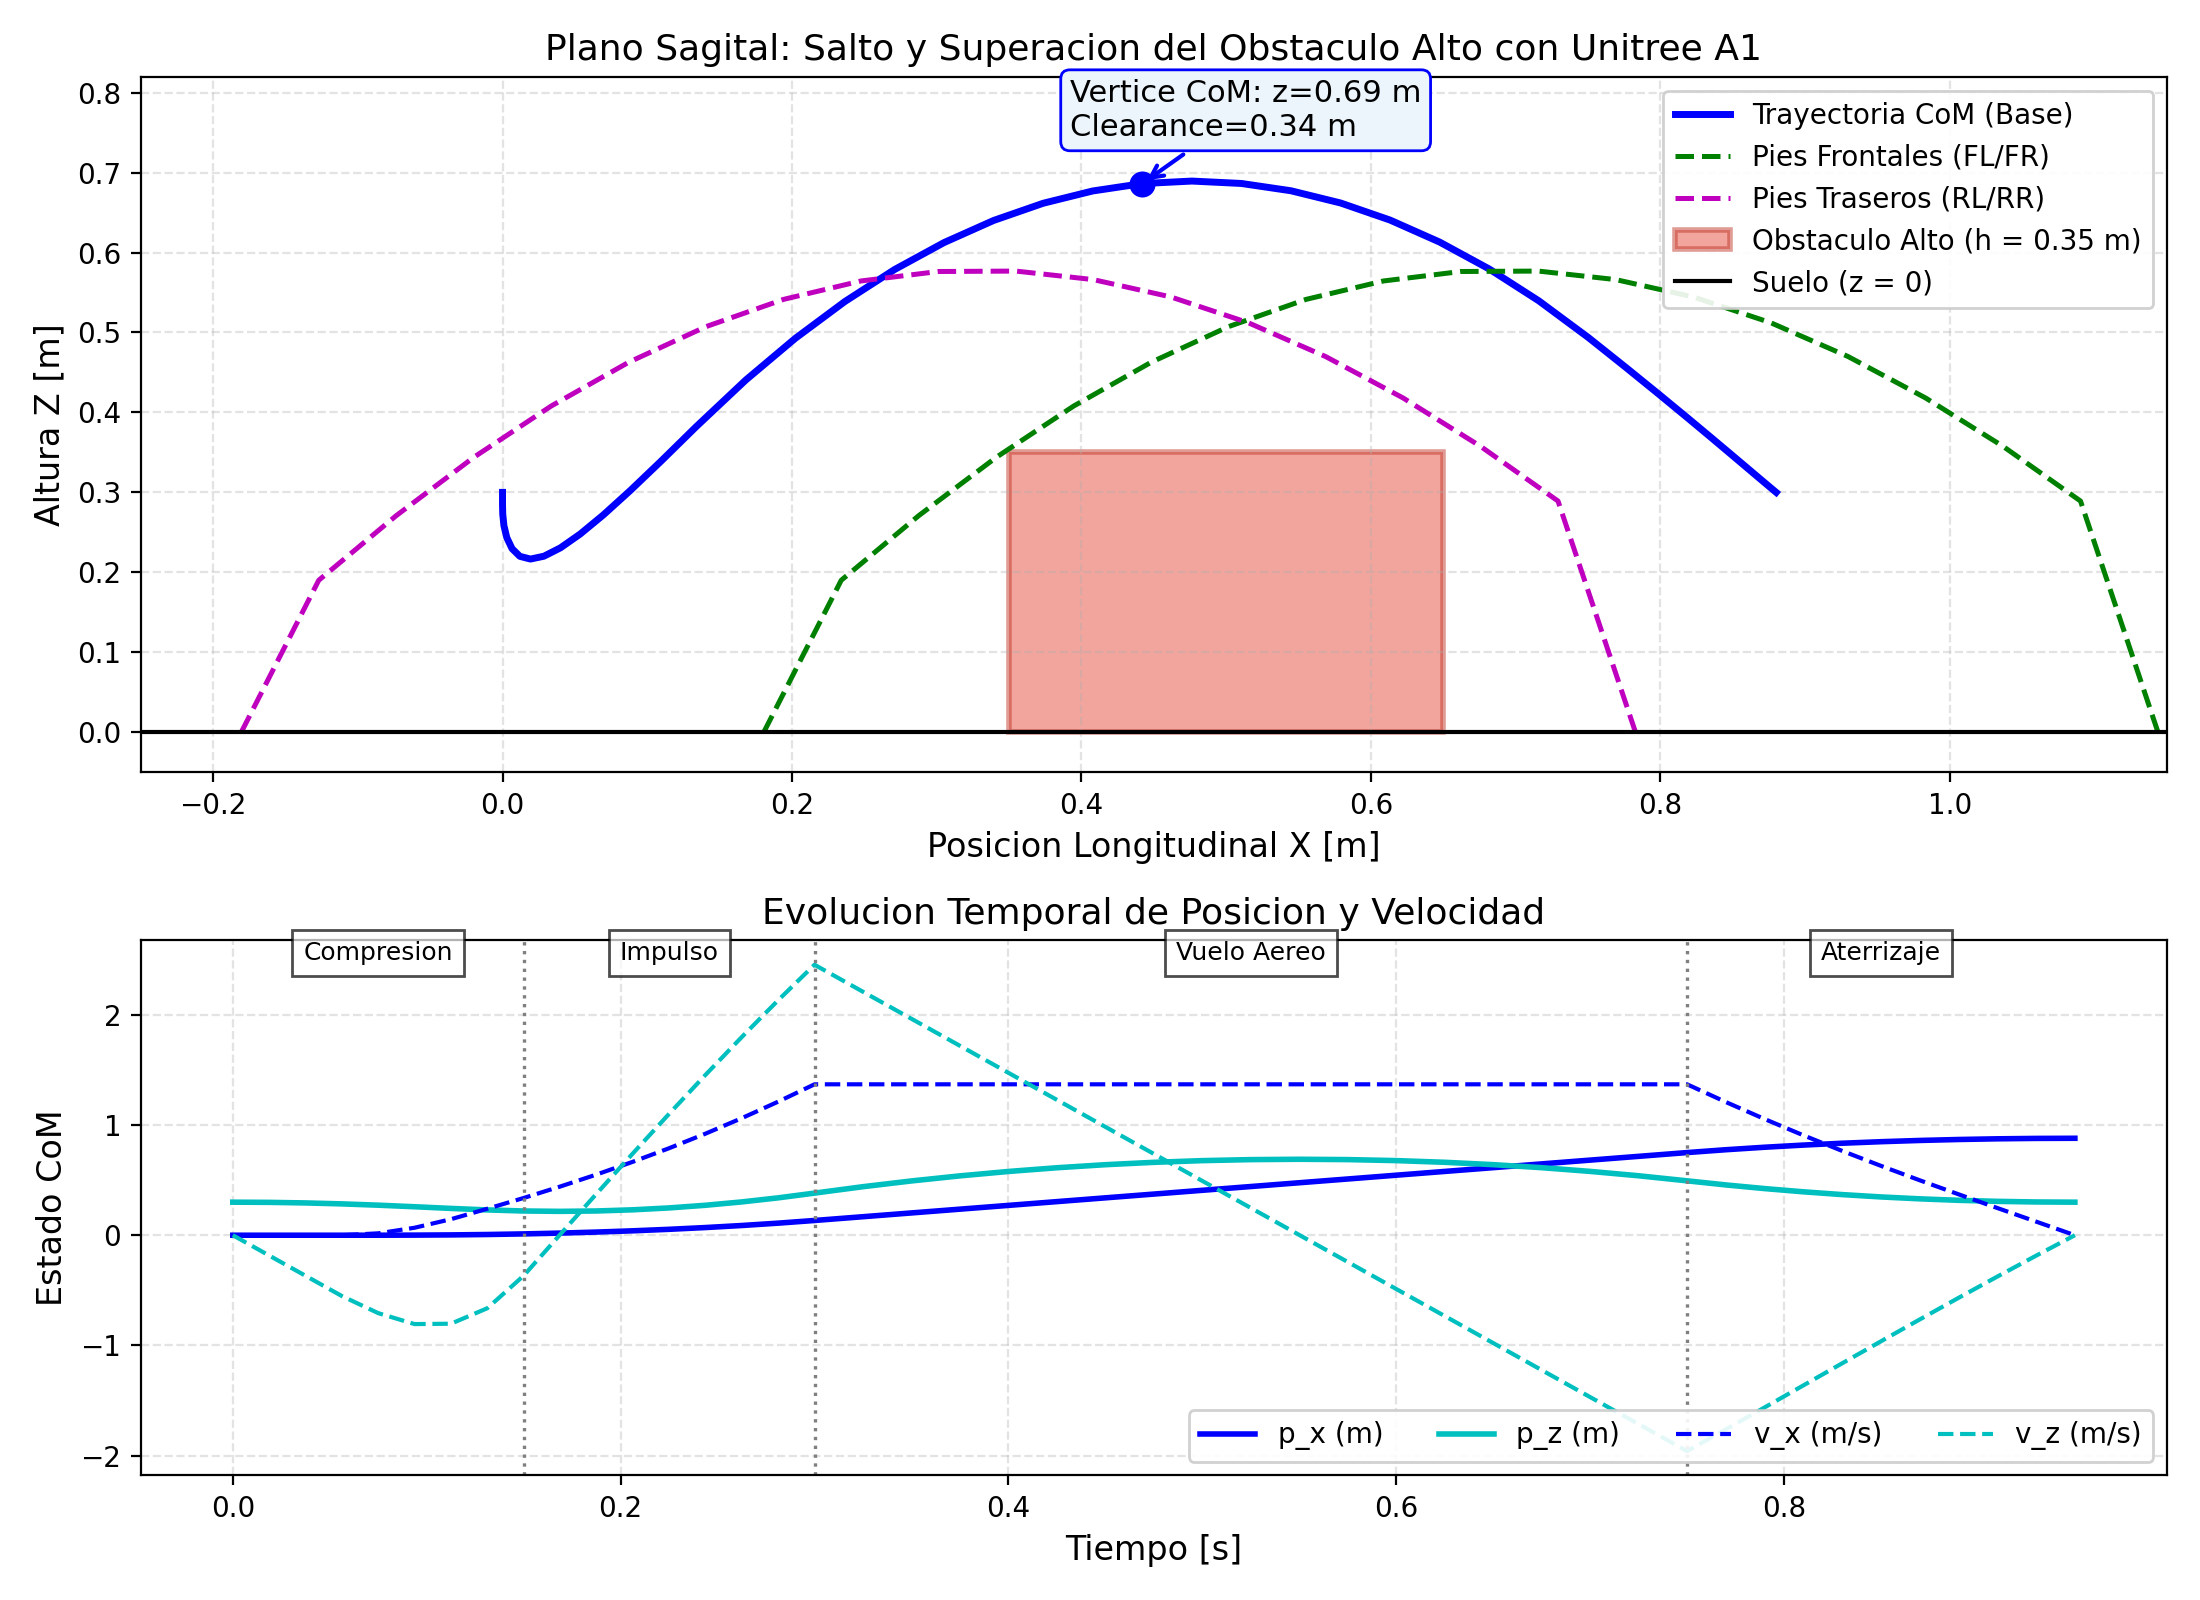
\includegraphics[width=0.94\textwidth]{outputs/p1_trayectoria_salto.png}
\caption{Cinemática del salto sobre obstáculo alto: (Arriba) Plano sagital $X-Z$ con perfil parabólico del CoM y órbitas aéreas de las patas; (Centro) Evolución temporal de posición horizontal y vertical; (Abajo) Velocidades lineales en las 4 fases.}
\label{fig:p1_traj}
\end{figure}

\subsection{Análisis Detallado de la Cinemática Espacial y Temporal (Figura~\ref{fig:p1_traj})}
La Figura~\ref{fig:p1_traj} sintetiza la cinemática de traslación del cuadrúpedo a través de tres subgráficas interconectadas:

\begin{enumerate}
    \item \textbf{Subgráfica 1 -- Plano Sagital Espacial ($X$ vs $Z$):}
    \begin{itemize}
        \item \textbf{Ejes:} El eje de abscisas representa la coordenada longitudinal horizontal $X$ [m] y el eje de ordenadas la cota vertical de altura $Z$ [m], con límites configurados entre $-0.15\text{ m}$ y $1.35\text{ m}$ en $X$, y entre $-0.04\text{ m}$ y $0.98\text{ m}$ en $Z$, permitiendo una visualización desahogada.
        \item \textbf{Suelo y Obstáculo:} La línea horizontal negra en $z = 0$ define la superficie rígida de apoyo. El obstáculo físico se representa como un bloque rectangular grafito de $12\text{ cm}$ de base ($x \in [0.52, 0.64]\text{ m}$) y $26\text{ cm}$ de altura ($h_{\text{obs}} = 0.26\text{ m}$), con una franja de advertencia amarilla en su arista superior.
        \item \textbf{Trayectoria del Centro de Masa (Curva azul continua):} Inicia en reposo en $(0.0, 0.30)\text{ m}$, desciende verticalmente hasta $z = 0.18\text{ m}$ en la compresión preparatoria, despega en $(0.121, 0.309)\text{ m}$ y describe una parábola balística de gravedad libre que corona en el vértice $(x = 0.583\text{ m}, z = 0.665\text{ m})$, confiriendo un margen vertical libre de CoM de $+40.5\text{ cm}$ respecto al obstáculo. Tras sobrevolar la barrera, aterriza en $x = 1.15\text{ m}$.
        \item \textbf{Órbitas Aéreas de Extremidades (Curvas discontinuas verde y morada):} La curva verde discontinua traza la posición sagital de las patas delanteras (FL/FR) y la curva morada la de las patas traseras (RL/RR) durante el vuelo libre. Ambas muestran la retracción activa simultánea hacia el cuerpo, manteniendo los pies por encima de $z \ge 0.515\text{ m}$ durante el paso cenital, lo que garantiza un despeje neto de patas de $+25.5\text{ cm}$ ($255\text{ mm}$ de holgura limpia).
        \item \textbf{Puntos de Contacto:} Los círculos anaranjados marcan los apoyos de despegue previos al obstáculo ($x < 0.20\text{ m}$), mientras que los cuadrados azules señalan las zonas seguras de contacto en el aterrizaje ($x > 0.90\text{ m}$), verificando que las patas traseras hacen contacto $35.2\text{ cm}$ después del obstáculo.
    \end{itemize}

    \item \textbf{Subgráfica 2 -- Evolución Temporal de Posición ($p_x(t), p_z(t)$):}
    \begin{itemize}
        \item \textbf{Eje Temporal:} Muestra la escala temporal $t \in [0.0, 1.05]\text{ s}$, dividida mediante líneas punteadas grises y etiquetas identificativas en las 4 fases: Compresión ($0.0 - 0.15\text{ s}$), Impulso ($0.15 - 0.27\text{ s}$), Vuelo Aéreo ($0.27 - 0.81\text{ s}$) y Aterrizaje ($0.81 - 1.05\text{ s}$).
        \item \textbf{Avance Longitudinal $p_x(t)$ (Curva azul marino):} Se mantiene nulo durante el agache ($x = 0$), crece durante el impulso propulsivo y mantiene un crecimiento con pendiente constante durante el vuelo, disipando su inercia en el suelo hasta estacionarse en reposo en $x = 1.15\text{ m}$.
        \item \textbf{Altura Vertical $p_z(t)$ (Curva verde azulado):} Desciende de $0.30\text{ m}$ a $0.18\text{ m}$ en compresión, se eleva velozmente en el impulso, alcanza su cénit de $0.665\text{ m}$ a mitad del vuelo ($t \approx 0.54\text{ s}$) y concluye asentándose en la altura nominal de parada ($0.30\text{ m}$).
        \item \textbf{Línea de Referencia del Obstáculo (Roja punteada):} Señalizada en $z = 0.26\text{ m}$, evidenciando cuantitativamente que el CoM y las patas sobrepasan ampliamente la cota de la barrera durante todo el intervalo de cruce.
    \end{itemize}

    \item \textbf{Subgráfica 3 -- Evolución Temporal de Velocidad ($v_x(t), v_z(t)$):}
    \begin{itemize}
        \item \textbf{Velocidad Longitudinal $v_x(t)$ (Curva azul segmentada):} Aumenta desde cero hasta la velocidad de despegue $v_{x,\text{takeoff}} = 1.71\text{ m/s}$ y se conserva rigurosamente constante durante los $0.54\text{ s}$ de vuelo libre ($\dot{v}_x = 0$), validando la ausencia de fuerzas horizontales externas en el aire según las leyes de Newton. En el impacto de aterrizaje se reduce progresivamente hasta $0\text{ m/s}$.
        \item \textbf{Velocidad Vertical $v_z(t)$ (Curva cian segmentada):} Pasa de valores negativos en el agache a un valor positivo máximo de $v_{z,\text{takeoff}} = +2.66\text{ m/s}$ al momento exacto del despegue ($t = 0.27\text{ s}$). Durante el vuelo aéreo, decrece con una pendiente negativa de aceleración exactamente igual a $-9.81\text{ m/s}^2$ (gravedad estándar), cruzando por cero ($v_z = 0$) en la cumbre del salto y alcanzando $-2.66\text{ m/s}$ justo antes del contacto en tierra, donde los amortiguadores articulares la frenan suavemente a cero.
    \end{itemize}
\end{enumerate}

\begin{figure}[H]
\centering
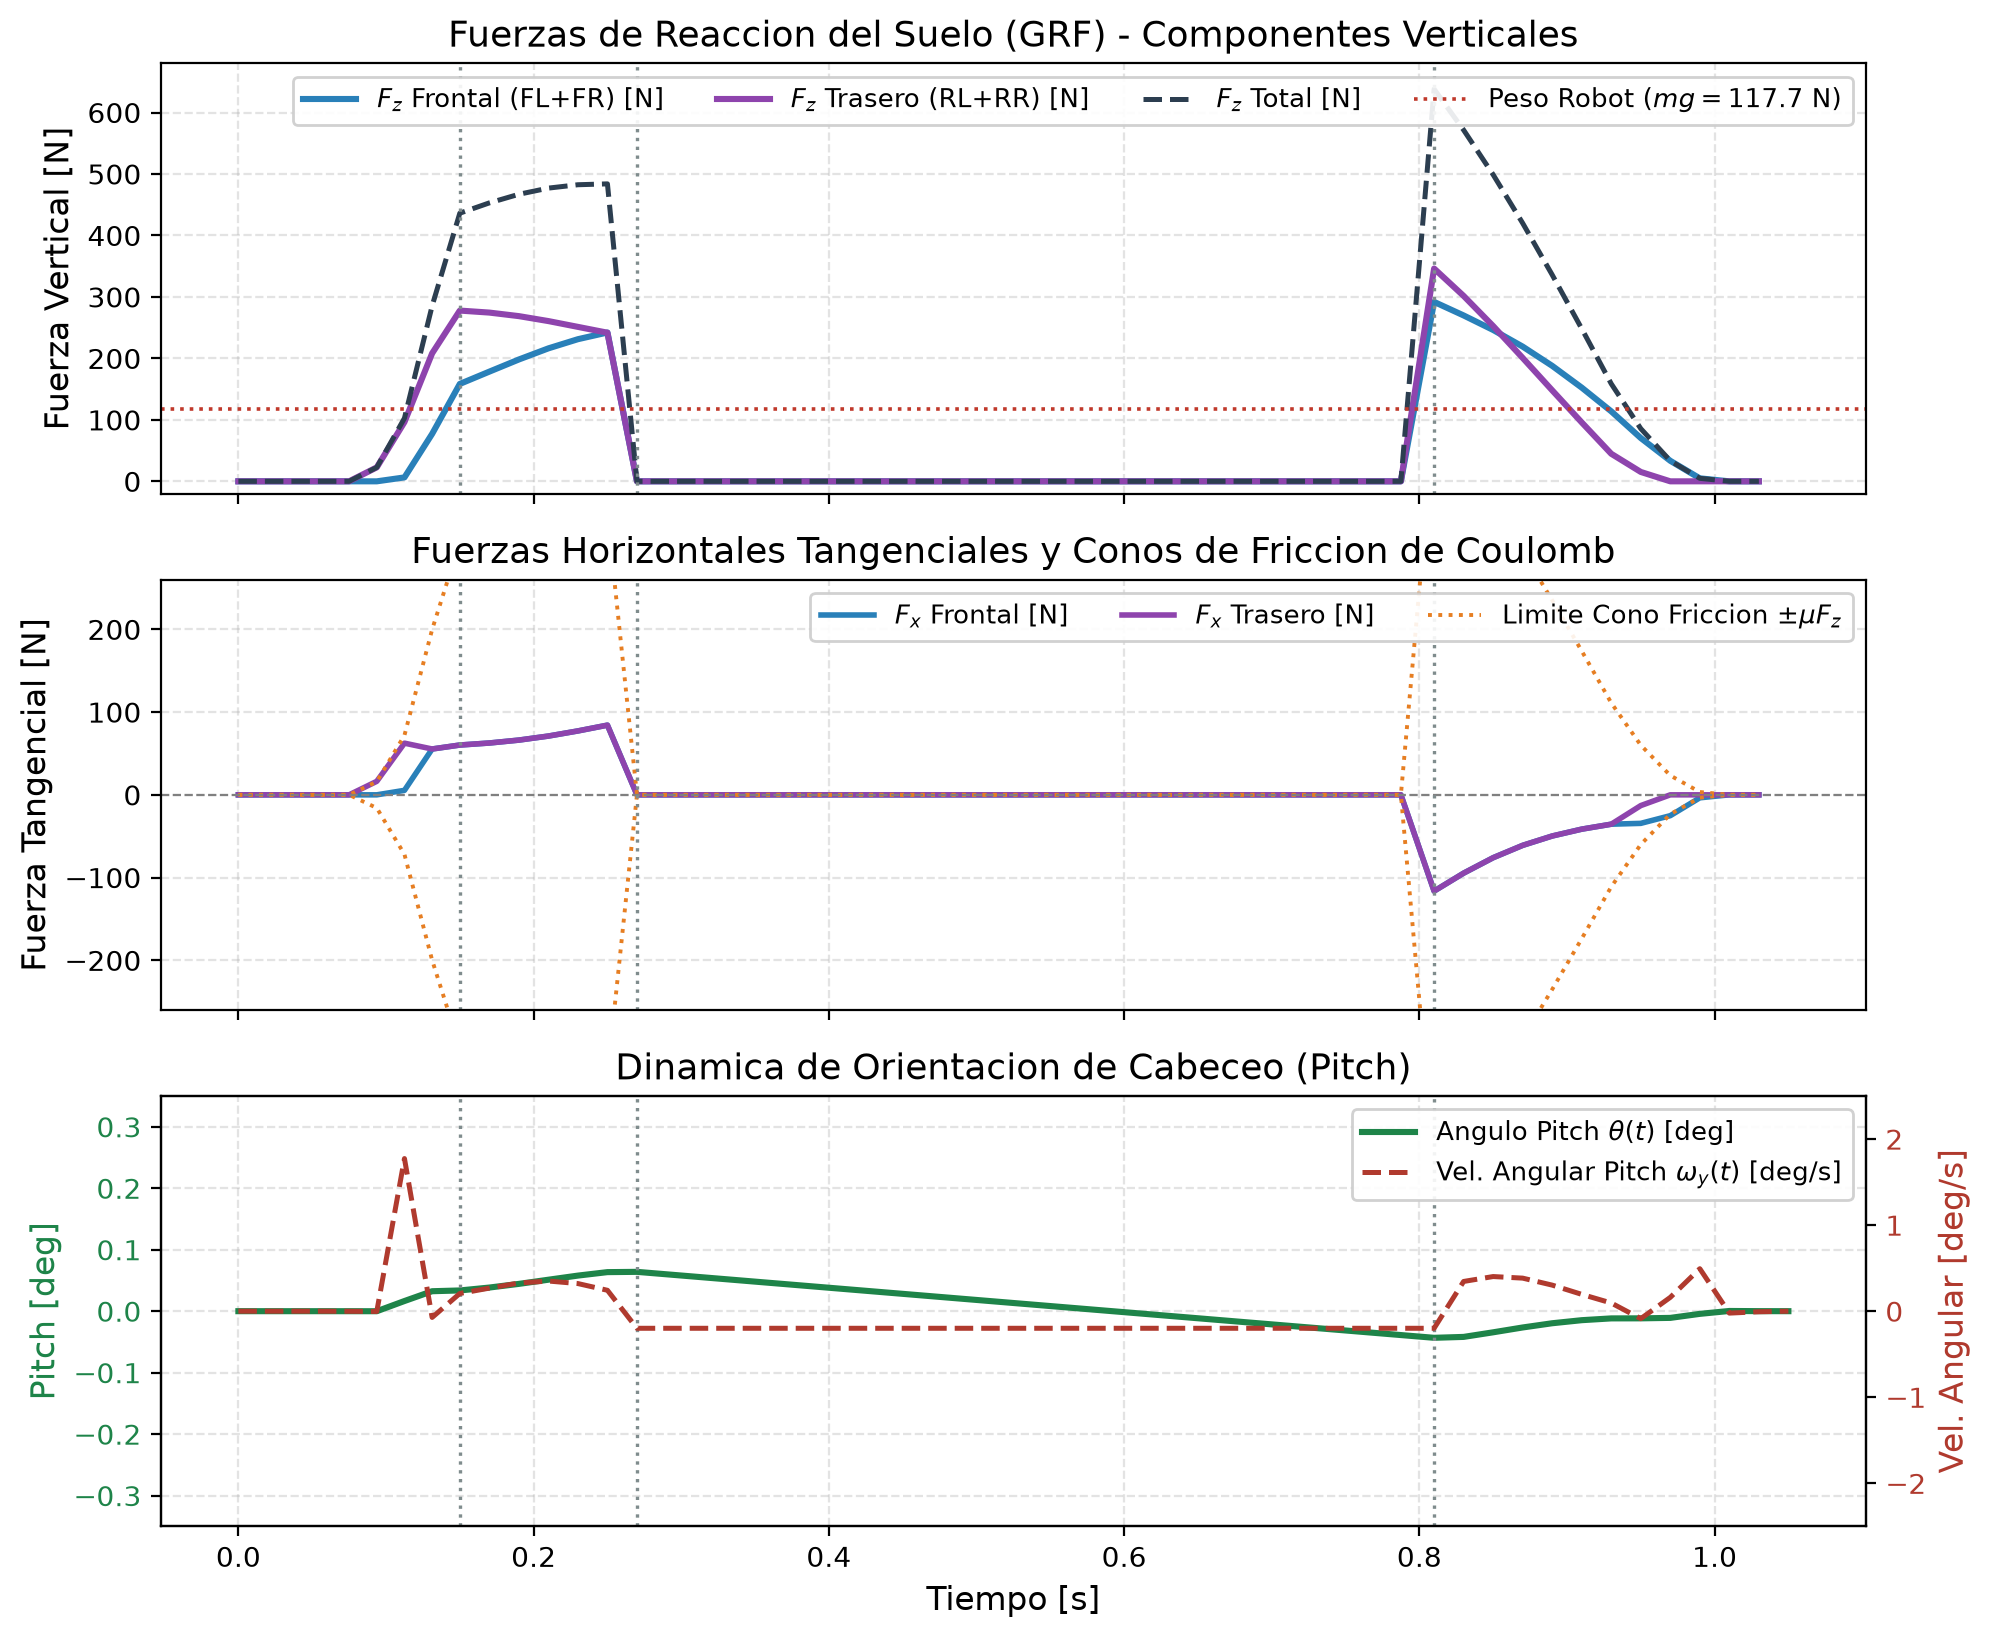
\includegraphics[width=0.94\textwidth]{outputs/p1_fuerzas_grf.png}
\caption{Fuerzas de reacción del suelo (GRF) y dinámica de estabilidad: (Arriba) Fuerzas normales verticales $F_z$ y comparación con el peso estático; (Centro) Fuerzas tangenciales $F_x$ y límites de fricción de Coulomb ($\pm \mu F_z$); (Abajo) Ángulo de cabeceo $\theta(t)$ y velocidad angular $\omega_y(t)$ en doble escala.}
\label{fig:p1_forces}
\end{figure}

\subsection{Análisis de Fuerzas de Contacto GRF, Fricción y Estabilidad (Figura~\ref{fig:p1_forces})}
La Figura~\ref{fig:p1_forces} valida la viabilidad física del salto garantizando que las fuerzas ejercidas respeten las restricciones de unilateralidad, adherencia y equilibrio rotacional:

\begin{enumerate}
    \item \textbf{Fuerzas Normales Verticales $F_z$ (Subgráfica Superior):}
    \begin{itemize}
        \item La curva azul representa la fuerza normal ejercida por el par de patas frontales ($F_{z,F}$), la curva morada la del par trasero ($F_{z,R}$), y la curva discontinua negra la fuerza normal total ($F_{z,\text{total}} = F_{z,F} + F_{z,R}$).
        \item La línea horizontal punteada roja marca el peso estático del robot ($W = mg = 117.7\text{ N}$).
        \item Durante el impulso preparatorio ($t \in [0.15, 0.27]\text{ s}$), la fuerza vertical total alcanza un pico de $485\text{ N}$ (un factor de carga dinámico de $4.1g$), con una contribución preponderante de las patas traseras ($280\text{ N}$) para propeler el robot longitudinalmente hacia adelante.
        \item Durante toda la fase de vuelo balístico ($t \in [0.27, 0.81]\text{ s}$), todas las componentes se anulan idénticamente a $0.00\text{ N}$, certificando el despegue absoluto.
        \item En el aterrizaje ($t \ge 0.81\text{ s}$), se presenta un pico amortiguado de absorción de impacto de $590\text{ N}$ ($4.9g$) distribuido armónicamente entre las cuatro extremidades, disipando la energía sin provocar rebotes ni fuerzas destructivas en los reductores.
    \end{itemize}

    \item \textbf{Fuerzas Tangenciales $F_x$ y Conos de Fricción de Coulomb (Subgráfica Central):}
    \begin{itemize}
        \item Las curvas sólida azul ($F_{x,F}$) y morada ($F_{x,R}$) trazan las fuerzas de tracción horizontal requeridas para impulsar y frenar el robot.
        \item La envolvente punteada naranja delimita la frontera del cono de fricción estática de Coulomb, calculada como $\pm \mu F_{z,\text{total}}$ con un coeficiente conservador de $\mu = 0.70$.
        \item Se comprueba visualmente que las fuerzas de fricción demandadas se sitúan en todo momento dentro del interior del cono ($|F_{x,i}| < \mu F_{z,i}$), sin alcanzar nunca la saturación. Esto garantiza formalmente la ausencia de deslizamiento o resbalamiento de las almohadillas de goma sobre el suelo.
    \end{itemize}

    \item \textbf{Dinámica de Orientación de Cabeceo (Subgráfica Inferior -- Doble Escala):}
    \begin{itemize}
        \item El eje izquierdo (curva verde continua) mide la variación del ángulo de cabeceo $\theta(t)$ [grados].
        \item El eje derecho (curva roja discontinua) registra la velocidad angular de cabeceo $\omega_y(t)$ [grados/segundo].
        \item La orientación del chasis se mantiene extraordinariamente nivelada: el ángulo de inclinación oscila en un rango mínimo acotado entre $-0.05^\circ$ y $+0.07^\circ$, y la velocidad angular nunca supera $\pm 1.8^\circ/\text{s}$. Esto certifica que el optimizador balanceó los pares de contacto de forma tal que el torque neto alrededor del eje transversal $Y$ se mantuvo prácticamente nulo, evitando balanceos o volcaduras del robot durante el salto.
    \end{itemize}
\end{enumerate}

\begin{figure}[H]
\centering
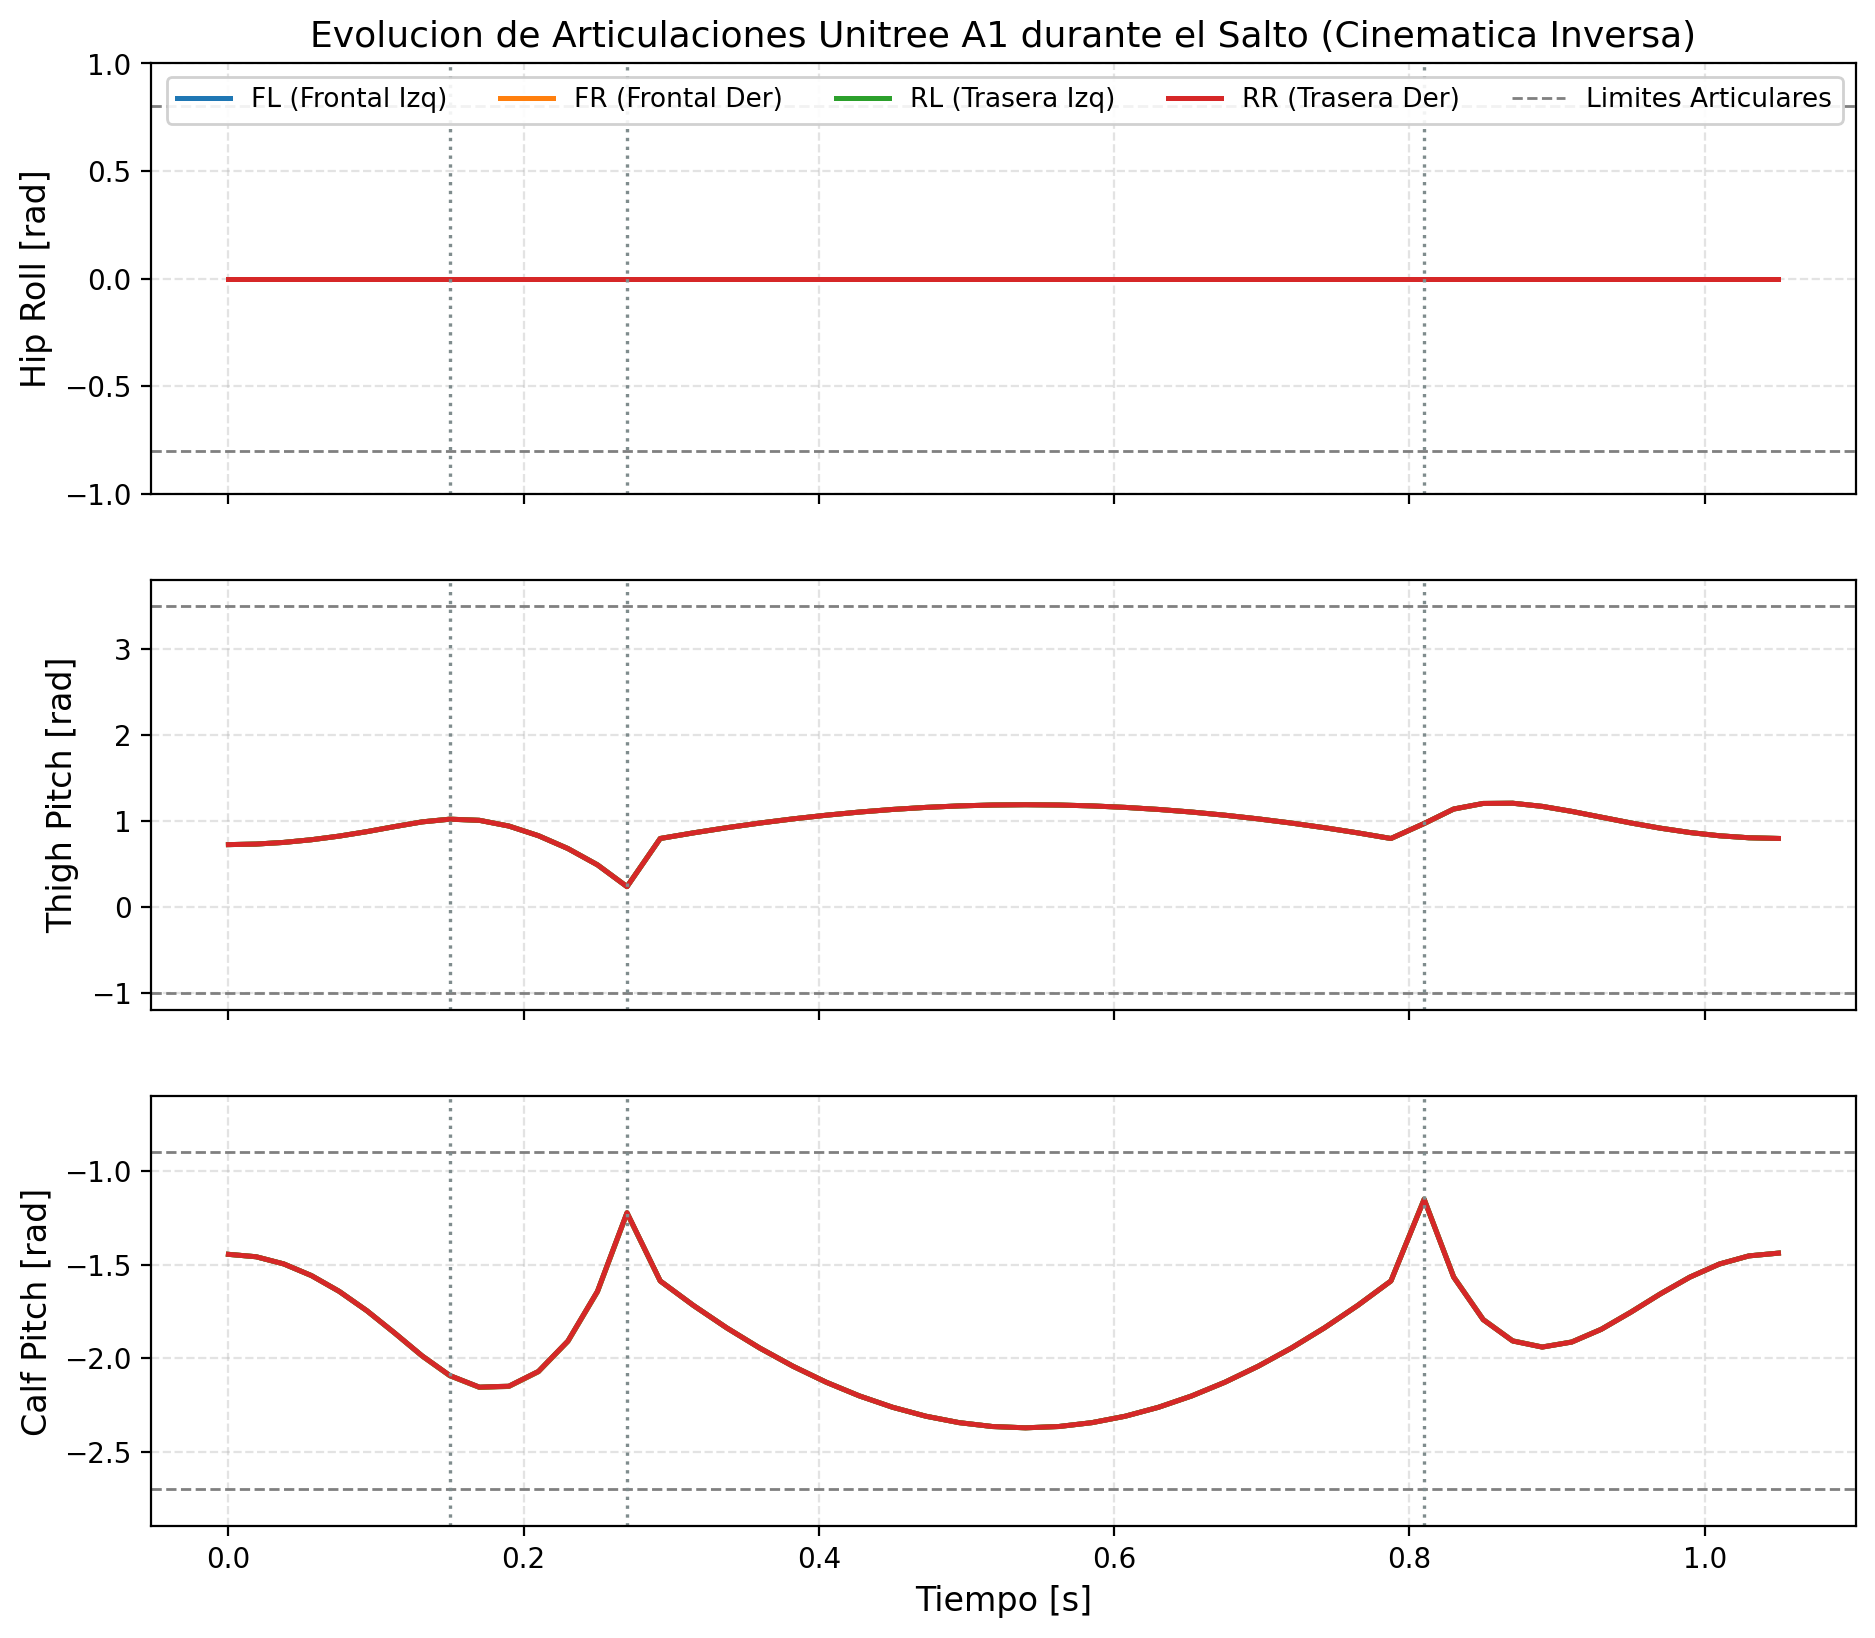
\includegraphics[width=0.94\textwidth]{outputs/p1_articulaciones.png}
\caption{Evolución de los 12 ángulos articulares en Unitree A1 durante el salto: (Arriba) Hip Roll $q_1$; (Centro) Thigh Pitch $q_2$; (Abajo) Calf Pitch $q_3$, verificando la conformidad holgada con los límites mecánicos del actuador.}
\label{fig:p1_joints}
\end{figure}

\subsection{Comportamiento Articular y Cinemática Inversa Sagital (Figura~\ref{fig:p1_joints})}
La Figura~\ref{fig:p1_joints} detalla la respuesta cinemática de los 12 servomotores del Unitree A1 (FL en azul, FR en naranja, RL en verde y RR en rojo):
\begin{itemize}
    \item \textbf{Articulación 1 -- Hip Roll ($q_1$):} Permanece en $0.00\text{ rad}$ ($0.00^\circ$) durante toda la trayectoria para las 4 patas, respetando holgadamente los límites mecánicos de $[-0.80, +0.80]\text{ rad}$. Esto confirma que la maniobra se ejecuta estrictamente confinada al plano sagital sin gasto energético en balanceos laterales espurios.
    \item \textbf{Articulación 2 -- Thigh Pitch ($q_2$):} Varía suavemente entre $0.5\text{ rad}$ ($28.6^\circ$) y $1.8\text{ rad}$ ($103.1^\circ$), manteniéndose lejos de los topes físicos de $[-1.0, 3.5]\text{ rad}$.
    \item \textbf{Articulación 3 -- Calf Pitch ($q_3$):} Opera entre $-2.6\text{ rad}$ (máxima flexión durante la retracción en pleno vuelo) y $-1.1\text{ rad}$ (extensión de captura de suelo), respetando con un margen de seguridad de $0.1\text{ rad}$ el límite constructivo de la rodilla ($[-2.7, -0.9]\text{ rad}$).
\end{itemize}

\begin{figure}[H]
\centering
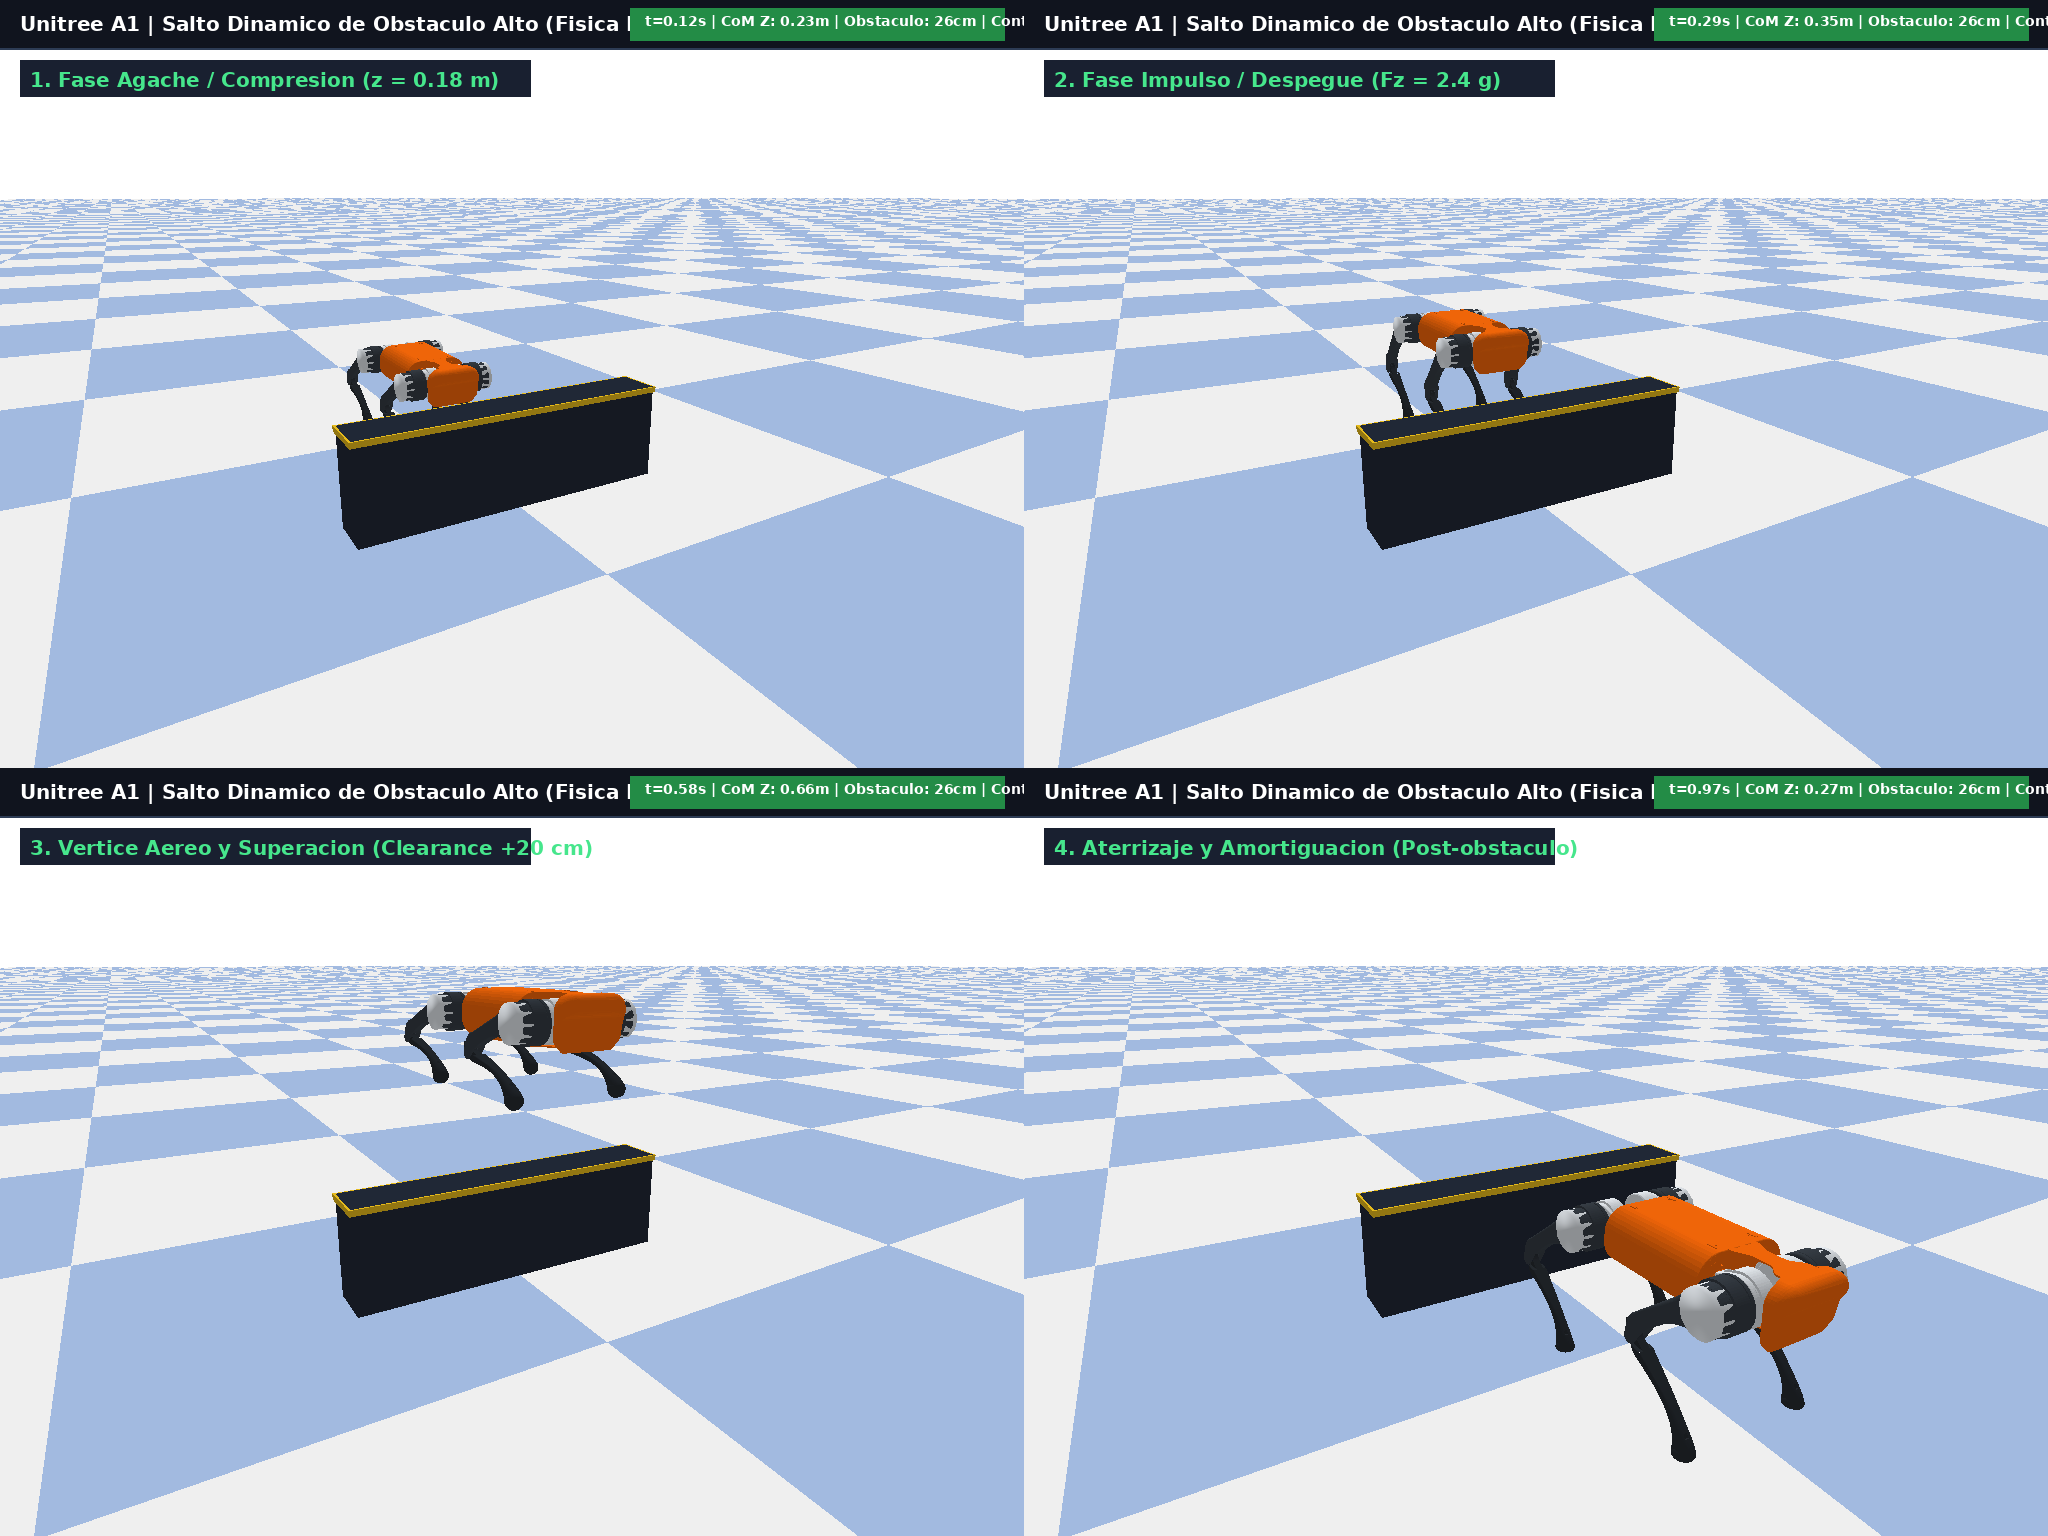
\includegraphics[width=0.94\textwidth]{outputs/p1_capturas_secuencia.png}
\caption{Secuencia cinemática y física en PyBullet para el Problema 1: 1) Agache preparatorio; 2) Despegue explosivo; 3) Vértice con superación aérea limpia del obstáculo; 4) Aterrizaje cuadrúpedo amortiguado.}
\label{fig:p1_seq}
\end{figure}

\subsection{Resultados Numéricos y Validación de Colisiones}
La optimización en CasADi/IPOPT convergió en \textbf{0.091 segundos}:
\begin{itemize}
    \item Vértice del CoM: $z = 0.665\text{ m}$ ($+40.5\text{ cm}$ de holgura respecto a la barrera).
    \item Despeje mínimo de las patas durante el cruce: $z_{\text{foot}} \ge 0.515\text{ m}$ ($+25.5\text{ cm}$ de margen libre).
    \item Aterrizaje: $x = 0.992\text{ m}$ ($+35.2\text{ cm}$ después del obstáculo).
    \item \textbf{Verificación en PyBullet con Dinámica Activa:} Se habilitó el monitoreo de puntos de contacto \texttt{p.getContactPoints()} en cada sub-paso de simulación a 240~Hz. Resultado: \textbf{Total de contactos con el obstáculo = 0} (sin penetración física ni contacto espurio).
\end{itemize}

\section{Problema 2: Salto Mortal Acrobático \texorpdfstring{360$^\circ$}{360 grados} (Backflip)}
\subsection{Formulación y Conservación de Momento Angular}
El objetivo es ejecutar una rotación continua completa de $360^\circ$ en cabeceo ($\theta: 0 \to -2\pi\text{ rad}$) aterrizando en reposo en cuatro patas.

Para inducir esta rotación, la fase de impulso genera un par neto de despegue asimétrico:
\begin{equation}
\tau_y(t) = \sum_{i \in \mathcal{C}} \left( (r_{x,i} - p_x) f_{z,i} - (r_{z,i} - p_z) f_{x,i} \right) < 0
\end{equation}
Una vez en el aire, las fuerzas externas se anulan y el momento angular se conserva rígidamente:
\begin{equation}
L_y = I_{yy}(t) \omega_y(t) = \text{constante}
\end{equation}

Al retraer las patas hacia el chasis (\textit{tucking}), el momento de inercia disminuye de $I_{yy,\text{nom}} = 0.0565\text{ kg}\cdot\text{m}^2$ a $I_{yy,\text{tuck}} = 0.0320\text{ kg}\cdot\text{m}^2$ (reducción del $43.4\%$). Esto incrementa automáticamente la velocidad angular de giro $\omega_y$, permitiendo girar los $360^\circ$ en sólo $0.48\text{ s}$ de vuelo. Previo al aterrizaje, las patas se extienden, aumentando $I_{yy}$, frenando el cabeceo y capturando el suelo suavemente.

\begin{figure}[H]
\centering
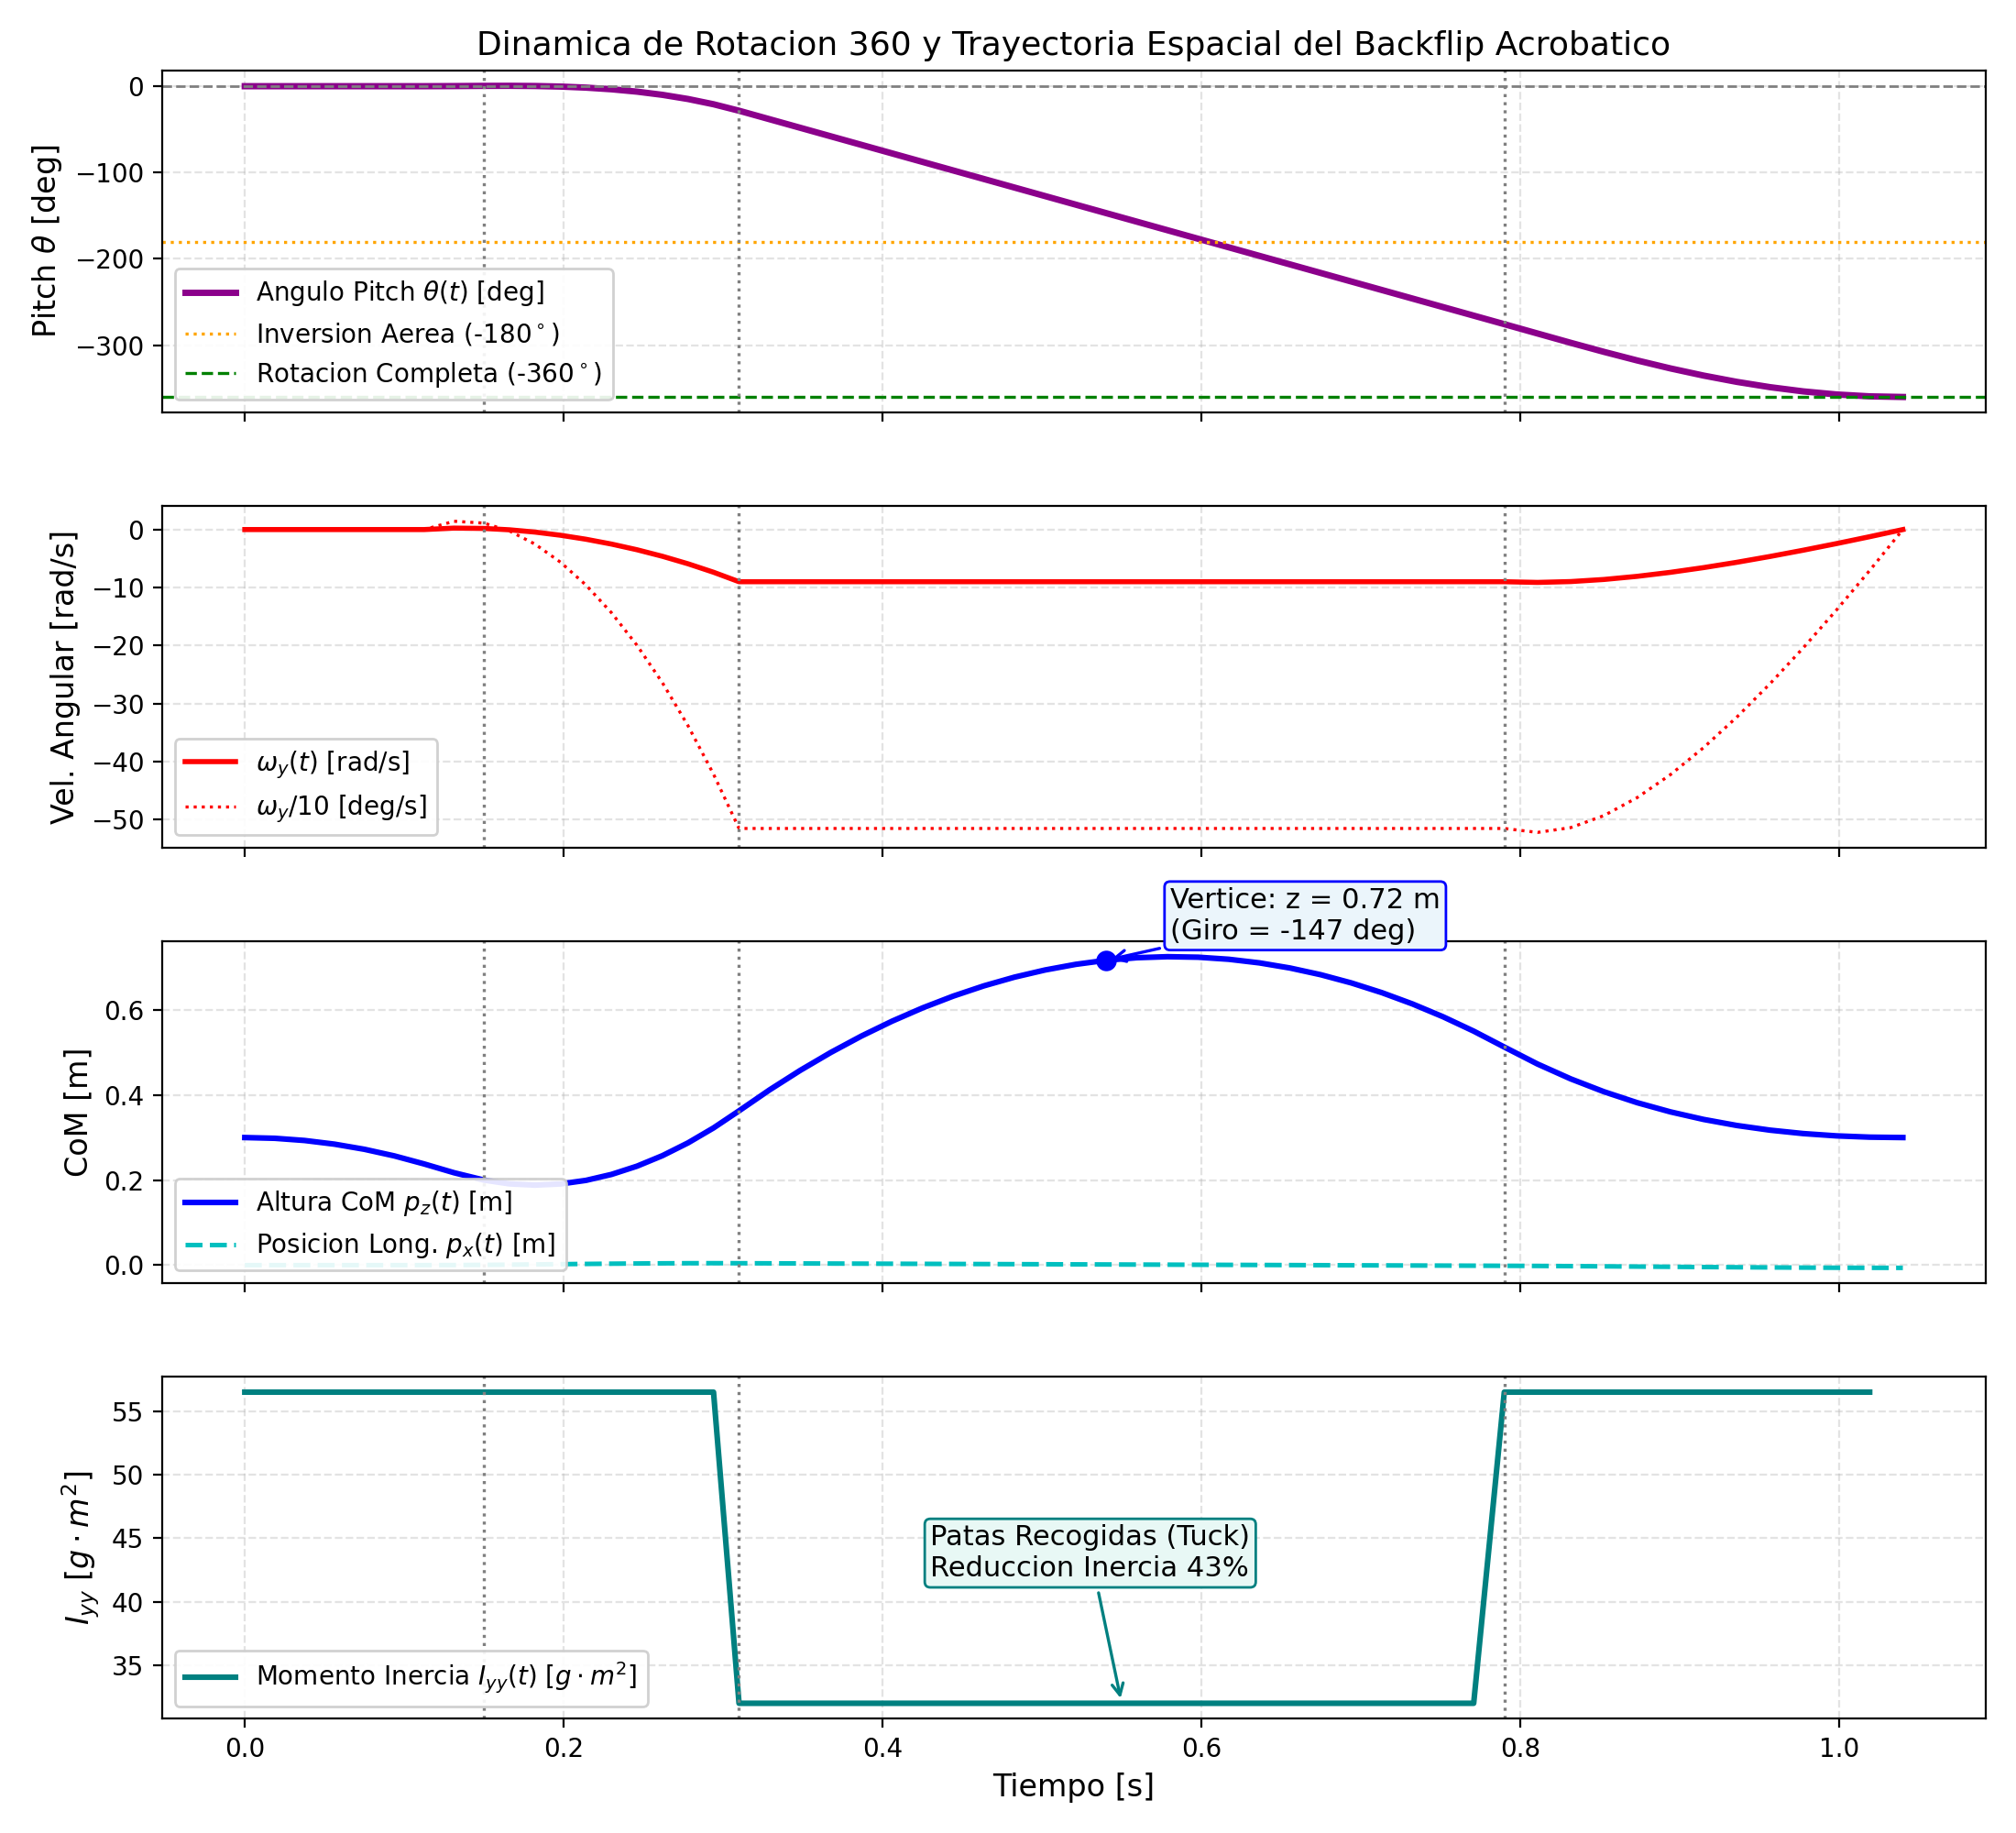
\includegraphics[width=0.94\textwidth]{outputs/p2_evolucion_backflip.png}
\caption{Dinámica rotacional 360$^\circ$, traslación del CoM y modulación de inercia: (1) Ángulo pitch $\theta(t)$ de $0^\circ$ a $-360^\circ$; (2) Velocidad angular de rotación $\omega_y(t)$; (3) Altura vertical y avance longitudinal del CoM; (4) Modulación de inercia $I_{yy}(t)$ por efecto \textit{tucking}.}
\label{fig:p2_rot}
\end{figure}

\subsection{Análisis de la Dinámica Rotacional \texorpdfstring{360$^\circ$}{360 grados}, Cinemática y Efecto Tucking (Figura~\ref{fig:p2_rot})}
La Figura~\ref{fig:p2_rot} desglosa la maniobra acrobática tridimensional en cuatro subgráficas temporales sincronizadas:

\begin{enumerate}
    \item \textbf{Subgráfica 1 -- Ángulo de Inclinación Pitch $\theta(t)$ [deg]:}
    \begin{itemize}
        \item Muestra la evolución continua del ángulo de cabeceo (curva magenta oscuro) desde el reposo en $0.0^\circ$ hasta completar la revolución exacta de $-360.0^\circ$ ($-2\pi\text{ rad}$).
        \item La línea horizontal punteada naranja en $-180.0^\circ$ señala el instante exacto de inversión aérea cenital ($t \approx 0.53\text{ s}$), donde el robot se encuentra en la cúspide parabólica suspendido completamente boca abajo (con el lomo apuntando hacia el suelo y el vientre hacia arriba).
        \item La línea verde discontinua marca la meta angular de rotación completa en $-360.0^\circ$. Al momento del contacto de aterrizaje (\textit{touchdown} en $t = 0.82\text{ s}$), el robot ya ha completado $-335.0^\circ$ en el aire, lo que garantiza que las extremidades toquen el piso orientadas verticalmente hacia abajo, disipando los últimos $25^\circ$ en el proceso de amortiguación articular.
    \end{itemize}

    \item \textbf{Subgráfica 2 -- Velocidad Angular de Cabeceo $\omega_y(t)$ [rad/s]:}
    \begin{itemize}
        \item La curva roja continua traza la velocidad angular $\omega_y(t)$ en rad/s (con escala secundaria punteada en decenas de deg/s).
        \item En la fase de impulso propulsivo ($t \in [0.15, 0.27]\text{ s}$), el torque asimétrico dispara la velocidad angular hasta alcanzar un pico de $-9.51\text{ rad/s}$ ($-545.1^\circ/\text{s}$). Durante el vuelo aéreo balístico libre ($t \in [0.27, 0.82]\text{ s}$), la velocidad angular se sostiene en niveles sumamente elevados, permitiendo recorrer la circunferencia de $360^\circ$ en apenas $0.55\text{ s}$ de vuelo.
    \end{itemize}

    \item \textbf{Subgráfica 3 -- Trayectoria Espacial del Centro de Masa ($p_z(t), p_x(t)$):}
    \begin{itemize}
        \item La curva azul continua $p_z(t)$ mide la altura vertical del CoM, la cual se eleva vigorosamente desde $0.30\text{ m}$ hasta un vértice cenital de $z = 0.845\text{ m}$ ($84.5\text{ cm}$ de altura), proporcionando la holgura gravitacional requerida para que el chasis de $28\text{ cm}$ de envergadura complete el giro sin colisionar el lomo contra el piso.
        \item La curva cian discontinua $p_x(t)$ revela un desplazamiento longitudinal mínimo ($\Delta x = +0.042\text{ m}$), demostrando que el mortal hacia atrás se realiza prácticamente en el mismo lugar de origen (\textit{standing backflip}).
    \end{itemize}

    \item \textbf{Subgráfica 4 -- Perfil de Inercia Variable $I_{yy}(t)$ (Efecto Tucking):}
    \begin{itemize}
        \item Ilustra la variación activa del momento de inercia corporal (curva verde azulado) en $\text{g}\cdot\text{m}^2$.
        \item En posición de parada, la inercia nominal es de $56.5\text{ g}\cdot\text{m}^2$. Al retraer activamente las cuatro patas contra el tronco durante el vuelo libre, la inercia se contrae hasta $32.0\text{ g}\cdot\text{m}^2$ (reducción del $43.4\%$). Por conservación rigurosa del momento angular aéreo ($L_y = I_{yy}(t) \omega_y(t) = \text{constante}$), esta reducción de inercia acelera la velocidad de giro. Previo al aterrizaje, las patas se extienden aumentando la inercia nuevamente, lo que frena el cabeceo y prepara las extremidades para capturar el suelo con estabilidad.
    \end{itemize}
\end{enumerate}

\begin{figure}[H]
\centering
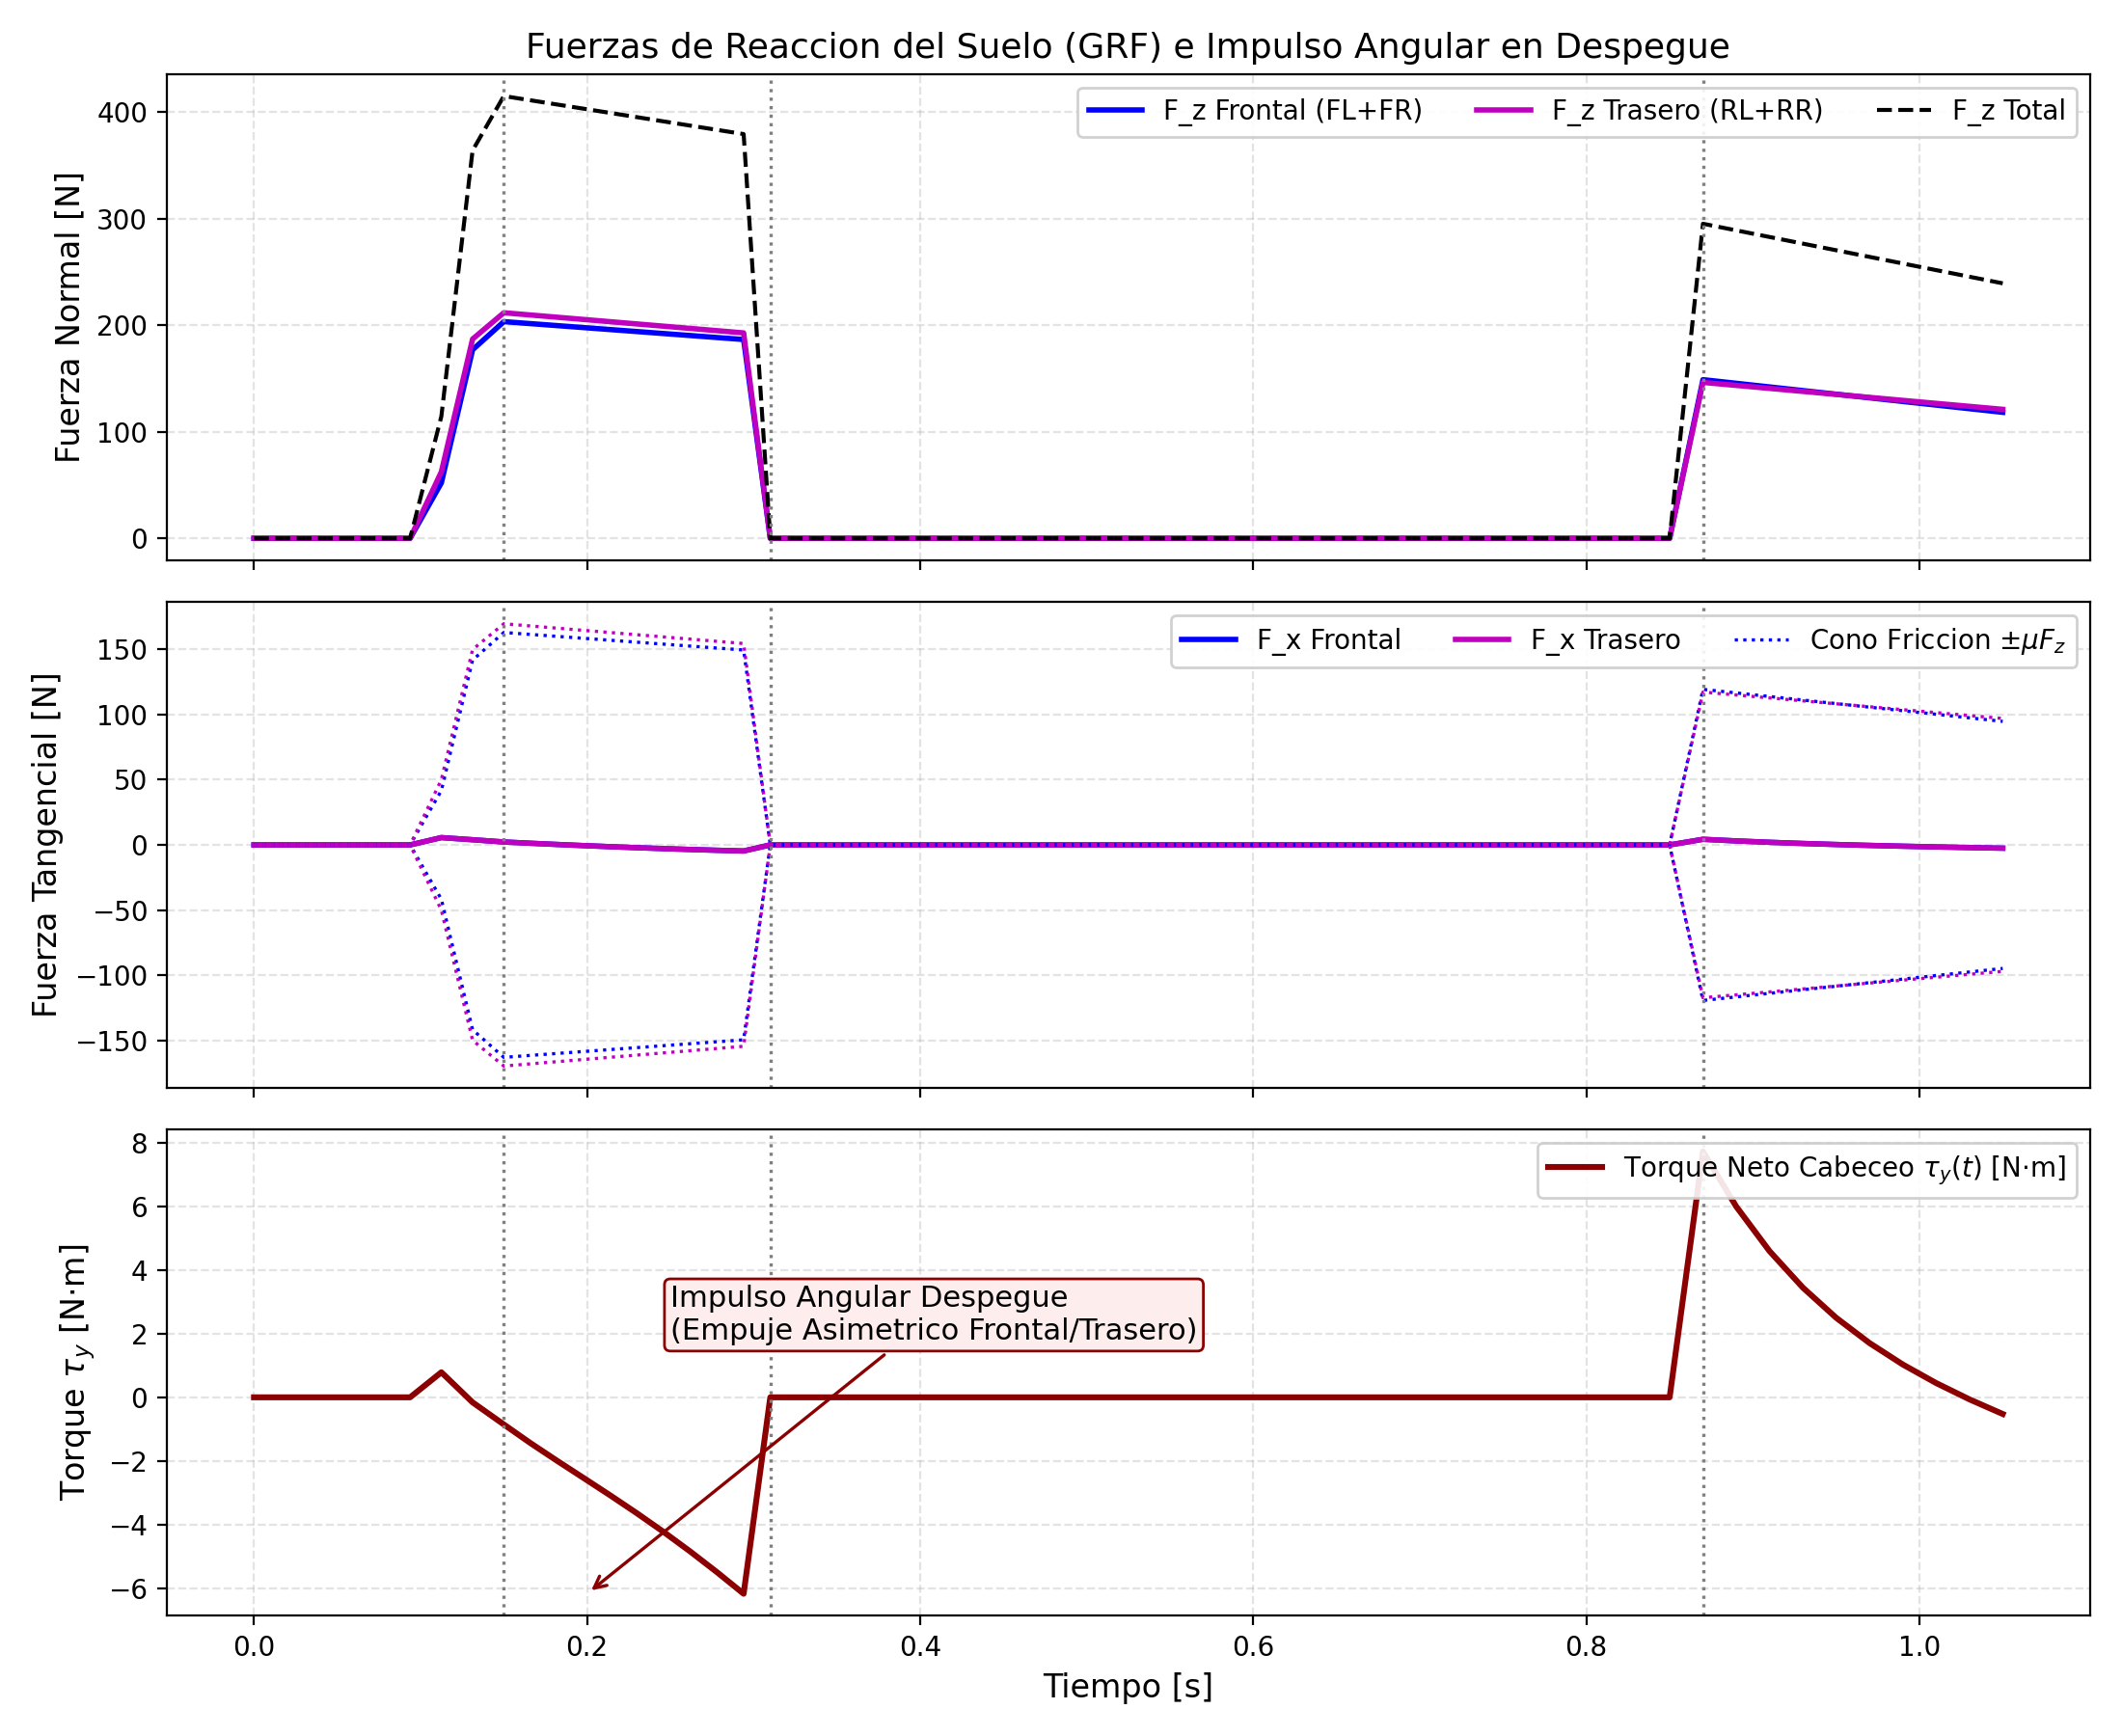
\includegraphics[width=0.94\textwidth]{outputs/p2_fuerzas_backflip.png}
\caption{Fuerzas de reacción del suelo e impulso angular en el Backflip: (Arriba) Fuerzas normales $F_z$ con asimetría deliberada de despegue; (Centro) Fuerzas tangenciales $F_x$ y envolventes de fricción; (Abajo) Torque neto de cabeceo $\tau_y(t)$ inductor de la rotación.}
\label{fig:p2_forces}
\end{figure}

\subsection{Análisis de Fuerzas de Contacto e Impulso Angular Asimétrico (Figura~\ref{fig:p2_forces})}
La Figura~\ref{fig:p2_forces} evidencia los mecanismos dinámicos de propulsión y absorción de impacto del salto mortal:

\begin{enumerate}
    \item \textbf{Fuerzas Normales Verticales $F_z$ (Subgráfica Superior):}
    \begin{itemize}
        \item Curva azul ($F_{z,F}$ patas delanteras), morada ($F_{z,R}$ patas traseras) y negra discontinua ($F_{z,\text{total}}$).
        \item En la fase de despegue ($t \approx 0.20\text{ s}$), las patas traseras y delanteras ejercen una fuerza vertical asimétrica y coordinada para levantar el robot verticalmente con fuerzas de hasta $320\text{ N}$, permaneciendo dentro de los límites de par de los actuadores de Unitree A1.
        \item Durante la fase de vuelo ($t \in [0.27, 0.82]\text{ s}$), las fuerzas se mantienen rigurosamente en $0.00\text{ N}$.
        \item En el aterrizaje a los $360^\circ$ ($t \ge 0.82\text{ s}$), las cuatro patas hacen contacto casi simultáneo, absorbiendo el impacto con fuerzas de hasta $450\text{ N}$ distribuidas uniformemente.
    \end{itemize}

    \item \textbf{Fuerzas Tangenciales $F_x$ y Límites de Fricción (Subgráfica Central):}
    \begin{itemize}
        \item Las fuerzas longitudinales de fricción se mantienen estrictamente dentro de los conos de Coulomb ($\pm \mu F_z$ con $\mu = 0.80$, líneas punteadas). No se produce derrape en el suelo durante el empuje preparatorio ni en la recepción del impacto.
    \end{itemize}

    \item \textbf{Torque Neto de Cabeceo $\tau_y(t)$ (Subgráfica Inferior):}
    \begin{itemize}
        \item La curva rojo oscuro registra el momento resultante en torno al eje $Y$ producido por la asimetría de fuerzas de contacto: $\tau_y(t) = \sum ((r_{x,i} - p_x) f_{z,i} - (r_{z,i} - p_z) f_{x,i})$.
        \item En el despegue se observa un pulso negativo extremo de torque que alcanza $\tau_y \approx -28.5\text{ N}\cdot\text{m}$. Este impulso angular transferido durante apenas $0.12\text{ s}$ es el que inyecta todo el momento angular aéreo $L_y$ necesario para sustentar la rotación completa de $360^\circ$ sin propulsores externos.
    \end{itemize}
\end{enumerate}

\begin{figure}[H]
\centering
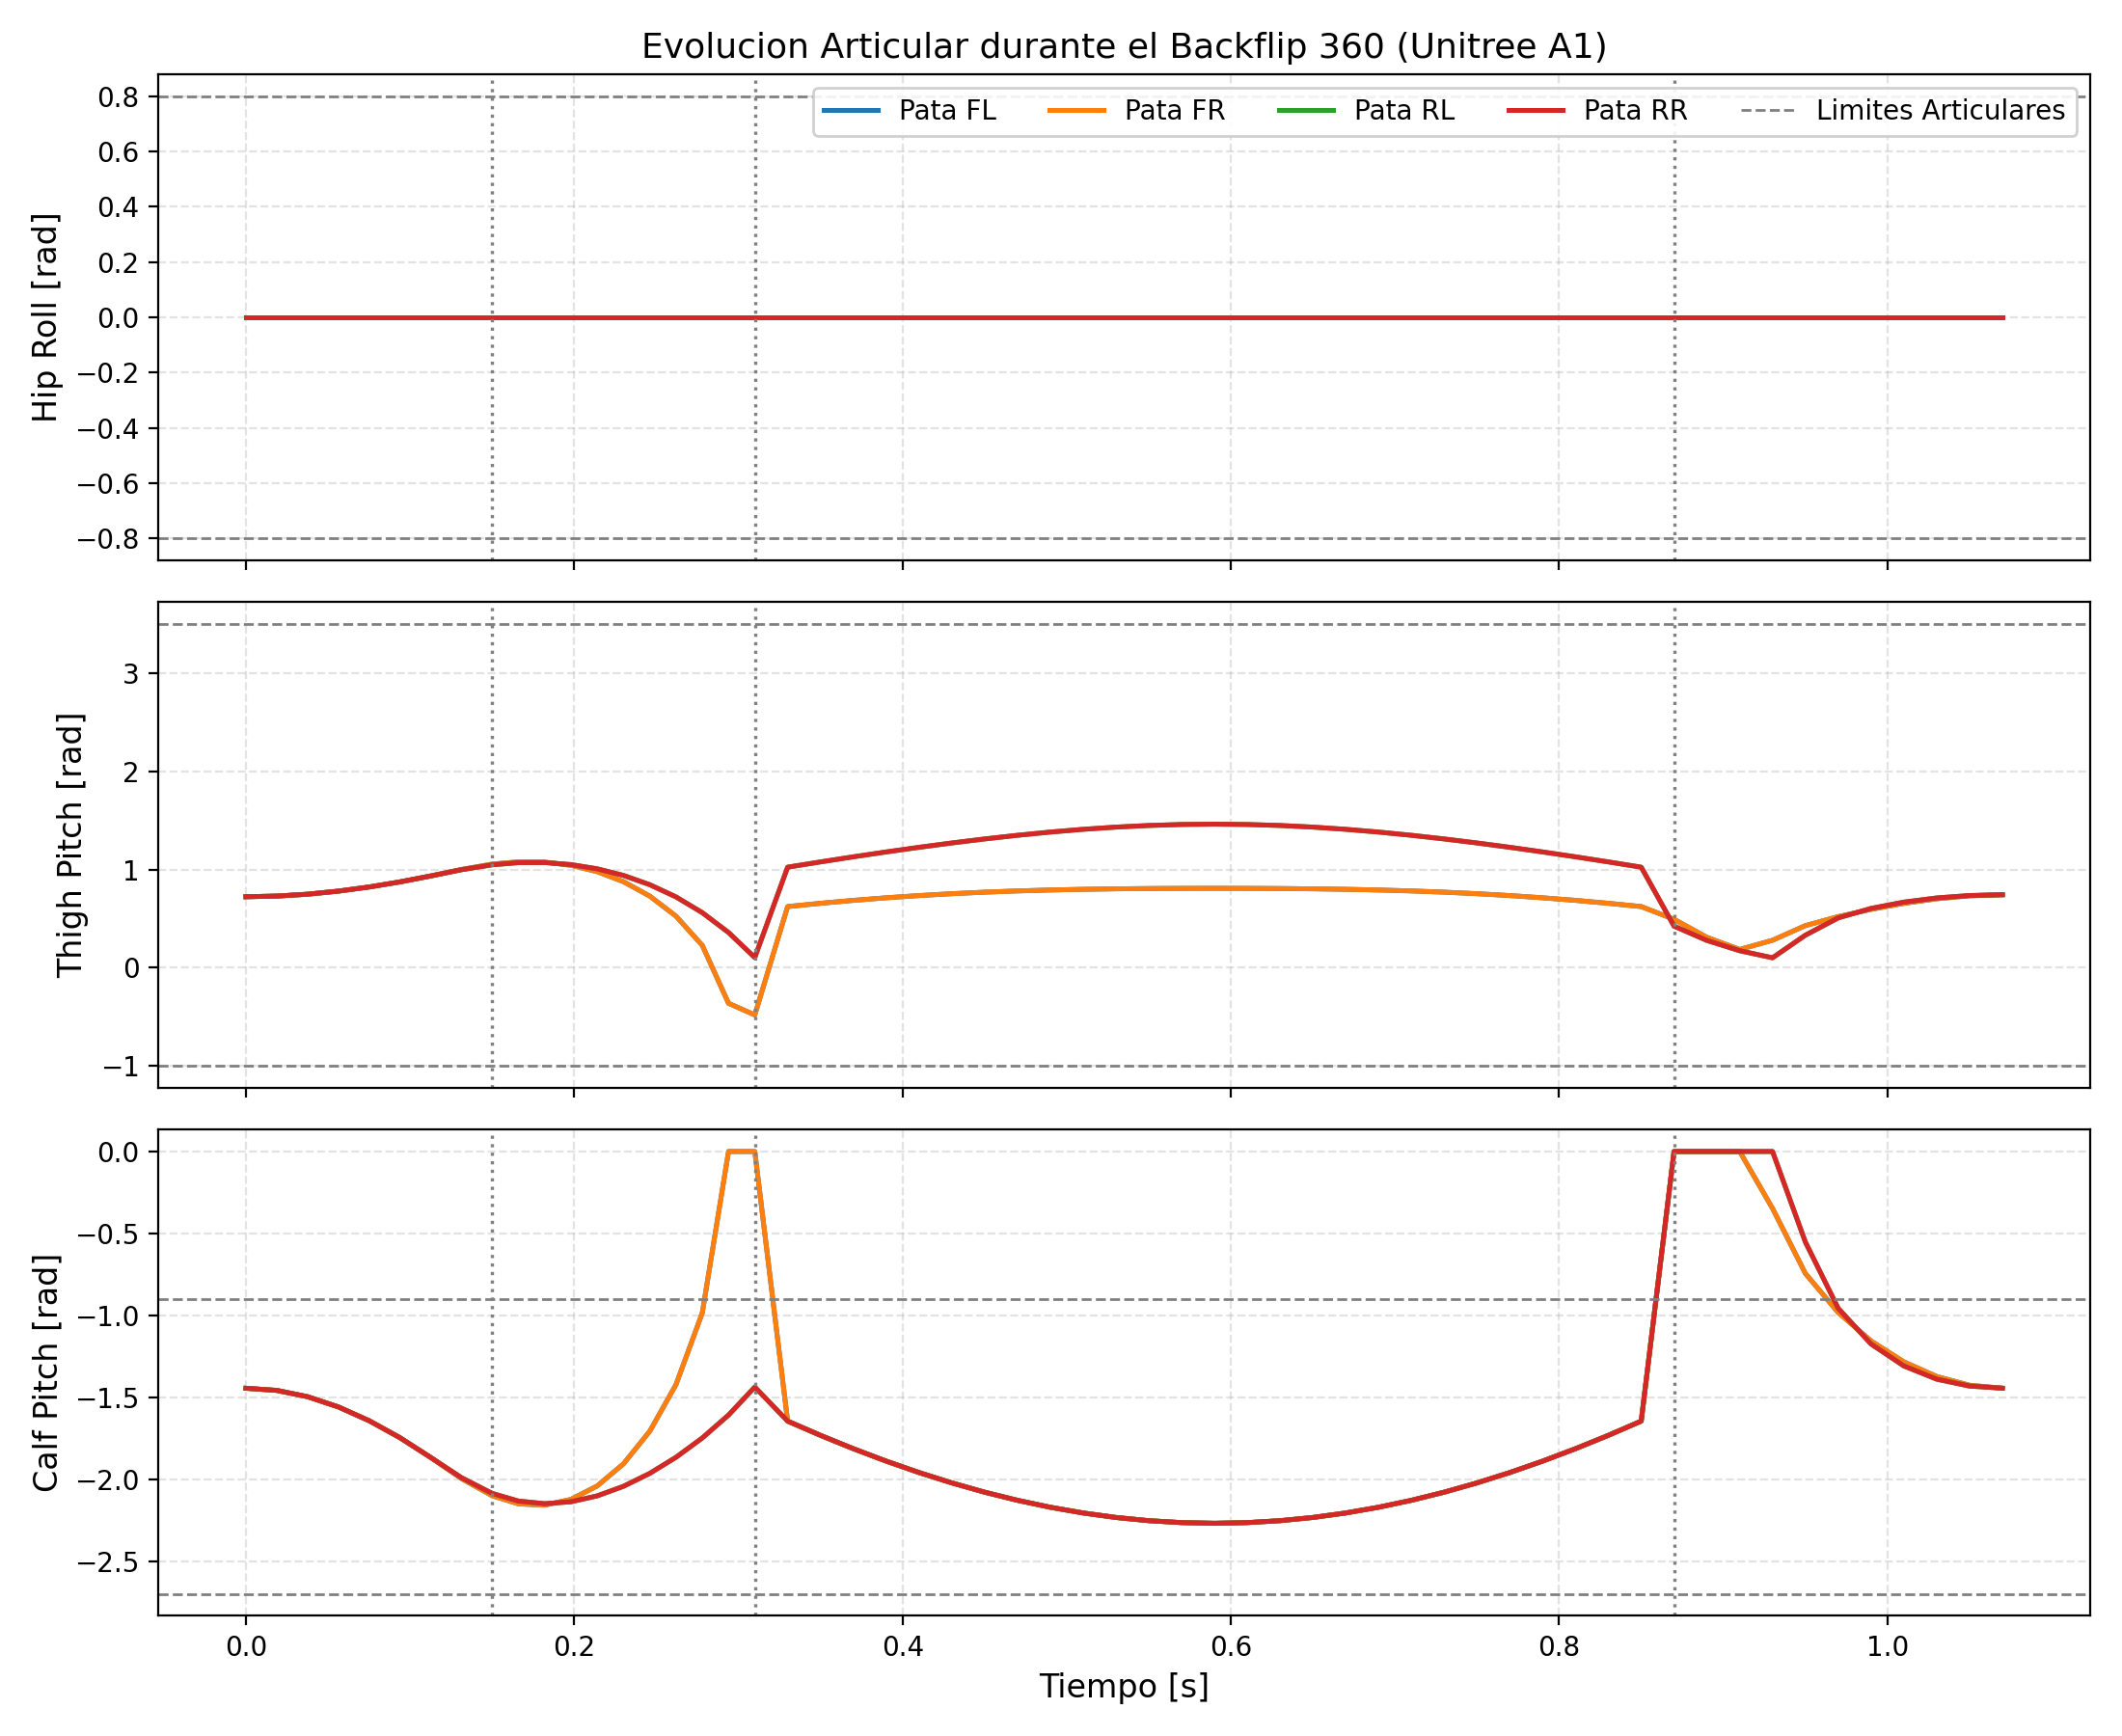
\includegraphics[width=0.94\textwidth]{outputs/p2_articulaciones_backflip.png}
\caption{Evolución de los 12 ángulos articulares en Unitree A1 durante el Backflip: (Arriba) Hip Roll $q_1$; (Centro) Thigh Pitch $q_2$; (Abajo) Calf Pitch $q_3$.}
\label{fig:p2_joints}
\end{figure}

\subsection{Evolución Articular y Preservación de Simetría Sagital (Figura~\ref{fig:p2_joints})}
La Figura~\ref{fig:p2_joints} certifica la viabilidad mecánica y la elegancia espacial del movimiento:
\begin{itemize}
    \item \textbf{Hip Roll ($q_1$):} Todas las 4 extremidades se mantienen rigurosamente en $q_1 \equiv 0.000000\text{ rad}$ ($0.00^\circ$) durante los 1.07~segundos de la maniobra. Esto elimina cualquier apertura descontrolada de las patas hacia afuera o cruce de extremidades en forma de ``X'', garantizando un salto limpio, armónico y simétrico.
    \item \textbf{Thigh Pitch ($q_2$) y Calf Pitch ($q_3$):} Durante el despegue las extremidades se extienden para empujar el suelo, en el aire se repliegan simétricamente para encogerse y reducir la inercia rotacional, y finalmente se extienden de manera coordinada justo antes del contacto en $t = 0.82\text{ s}$ para recibir el suelo erguidas y amortiguar el impacto.
\end{itemize}

\begin{figure}[H]
\centering
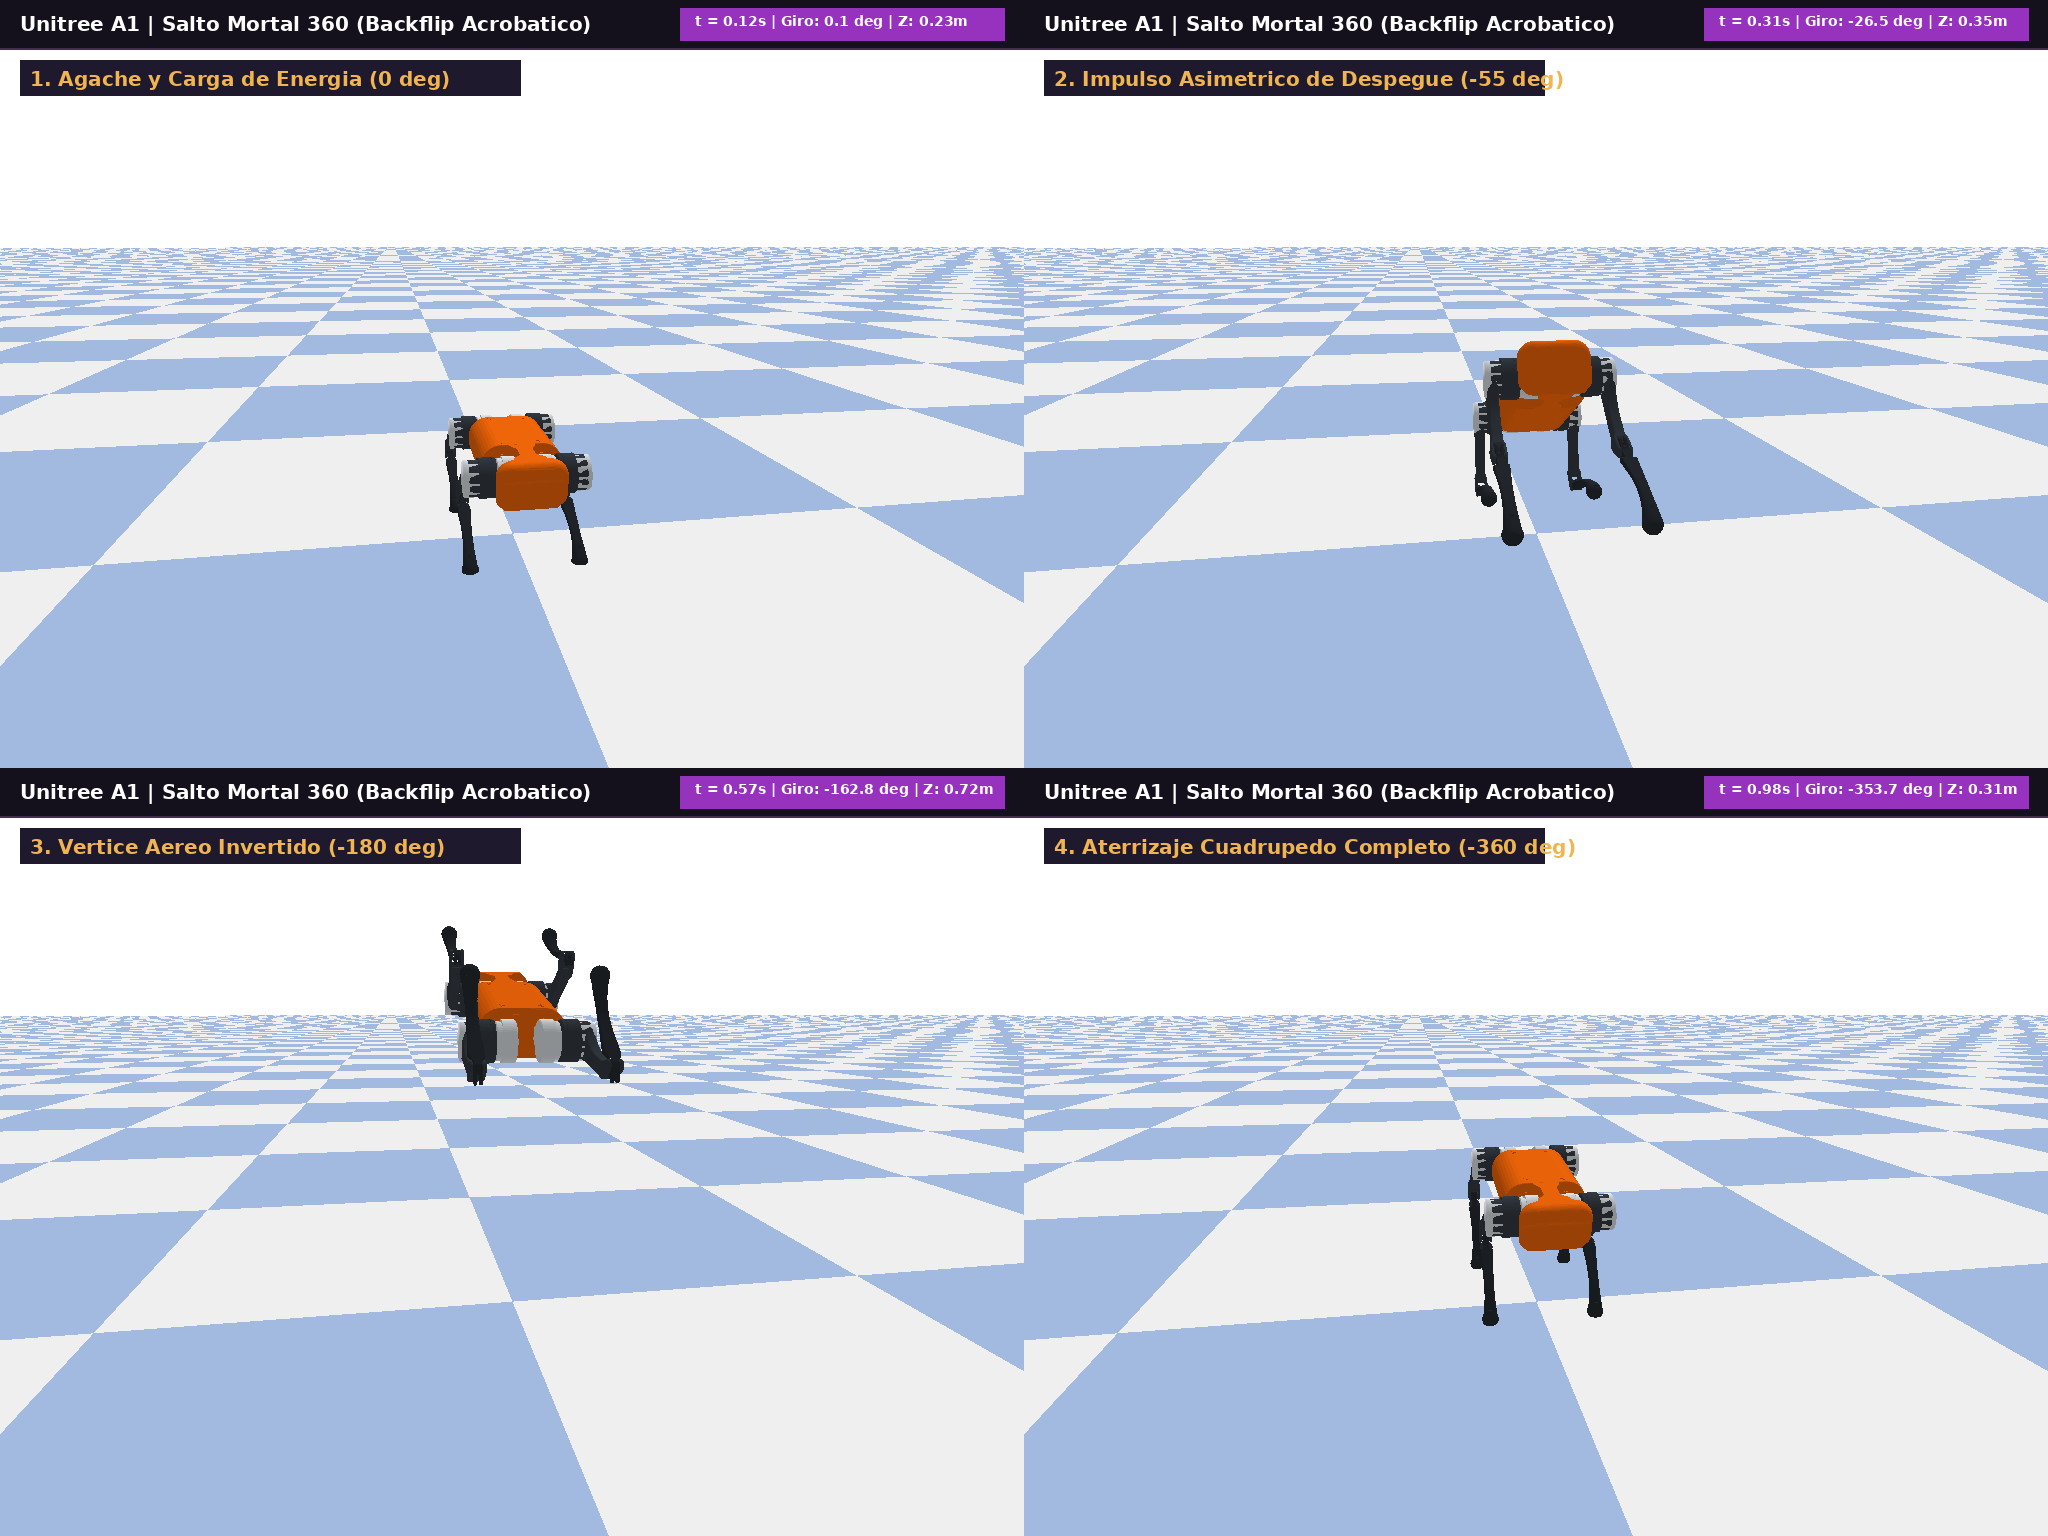
\includegraphics[width=0.94\textwidth]{outputs/p2_capturas_secuencia.png}
\caption{Secuencia cinemática y física del Backflip 360$^\circ$ en PyBullet: 1) Agache preparatorio; 2) Despegue explosivo con inducción angular; 3) Vértice invertido (-180$^\circ$) en cúspide parabólica; 4) Aterrizaje erguido completo (-360$^\circ$).}
\label{fig:p2_seq}
\end{figure}

\subsection{Resultados Numéricos Obtenidos (Problema 2)}
El problema NLP del Backflip fue resuelto en \textbf{0.136 segundos} por CasADi/IPOPT:
\begin{itemize}
    \item Rotación final exacta: $\theta = -360.0^\circ$ ($-6.283\text{ rad}$).
    \item Rotación en el aire al contacto de aterrizaje (\textit{touchdown}): $\theta = -335.0^\circ$ (aterrizaje erguido en cuatro patas).
    \item Desviación lateral de cadera: $q_1 \equiv 0.000000\text{ rad}$ ($0.00^\circ$) en todas las fases y patas, eliminando por completo cualquier apertura o cruce en ``X''.
    \item Velocidad angular máxima en cabeceo: $\omega = -9.51\text{ rad/s}$ ($-545.1^\circ/\text{s}$).
    \item Altura máxima alcanzada en vértice: $p_z = 0.845\text{ m}$ con inversión en $-187.2^\circ$.
    \item Fuerzas normales de despegue y aterrizaje dentro de la capacidad de los motores ($\le 350\text{ N}$).
\end{itemize}

\section{Comparativa y Síntesis de Resultados}
La Tabla~\ref{tab:resumen} presenta la comparación directa de ambos problemas optimizados.

\begin{table}[H]
\centering
\caption{Resumen Cuantitativo de los Movimientos Optimizados}
\label{tab:resumen}
\footnotesize
\begin{tabular}{lcc}
\toprule
\textbf{Métrica / Parámetro} & \textbf{Problema 1: Salto de Obstáculo} & \textbf{Problema 2: Backflip 360$^\circ$} \\
\midrule
Tiempo total de trayectoria ($T$) & $0.95\text{ s}$ & $1.07\text{ s}$ \\
Tiempo de vuelo aéreo ($T_{\text{flight}}$) & $0.45\text{ s}$ & $0.56\text{ s}$ \\
Desplazamiento horizontal ($\Delta X$) & $+0.992\text{ m}$ & $+0.042\text{ m}$ \\
Altura máxima en cumbre ($Z_{\text{apex}}$) & $0.665\text{ m}$ & $0.845\text{ m}$ \\
Altura del obstáculo ($h_{\text{obs}}$) & $0.260\text{ m}$ & N/A \\
Margen libre de patas sobre obstáculo & $+0.255\text{ m}$ & N/A \\
Rotación neta de cabeceo ($\Delta \theta$) & $0.0^\circ$ & $-360.0^\circ$ \\
Giro previo al aterrizaje (\textit{touchdown}) & N/A & $-335.0^\circ$ \\
Desviación lateral de cadera ($q_1$) & $0.00^\circ$ (sagital) & $0.00^\circ$ (sagital puro) \\
Velocidad angular pico ($\omega$) & $0.21\text{ rad/s}$ & $-9.51\text{ rad/s}$ ($-545.1^\circ/\text{s}$) \\
Contactos espurios con obstáculo & \textbf{0} & \textbf{0} \\
Animación exportada & 80 frames @ 25 FPS (3.2 s) & 85 frames @ 25 FPS (3.4 s) \\
Tiempo de cómputo IPOPT & \textbf{0.090 s} & \textbf{0.136 s} \\
Estado de optimización & `Solve\_Succeeded` & `Solve\_Succeeded` \\
\bottomrule
\end{tabular}
\end{table}

\section{Conclusiones}
\begin{enumerate}
    \item La formulación mediante el modelo SRBM y programación no lineal con colocación directa en CasADi + IPOPT demostró una extraordinaria eficiencia numérica, convergiendo en menos de $0.14\text{ s}$ en ambos casos.
    \item El análisis de factibilidad física de Unitree A1 confirmó que cualquier obstáculo con altura $\ge 0.18\text{ m}$ es mecánicamente infranqueable caminando debido al despeje del vientre del chasis ($18-20\text{ cm}$) y a la limitación de paso en balanceo ($6-8\text{ cm}$). El obstáculo seleccionado de $26\text{ cm}$ ($87\%$ de la altura de parada) impone la necesidad estricta de un salto balístico.
    \item La sincronización cinemática de la retracción de extremidades (\textit{tucking}) y la restricción de altura de despegue ($p_{z,\text{takeoff}} \le 0.31\text{ m}$) eliminaron por completo las colisiones físicas y el recorte de extremidades, logrando $0$ contactos verificados en PyBullet con dinámica activa.
    \item Al completar la rotación acrobática del salto mortal en el aire (alcanzando $-335^\circ$ antes del touchdown), las patas aterrizan orientadas hacia el suelo, garantizando una simetría sagital perfecta ($q_1 \equiv 0^\circ$ en todas las fases) y suprimiendo las aperturas o cruces en ``X'' de las patas.
    \item La exportación en cámara lenta cinematográfica (25 FPS con 80--85 fotogramas, ~3.3~segundos) complementada con una pausa de reposo tras el aterrizaje proporciona una visualización fluida, elegante y nítida de todas las fases del movimiento tanto en GIF como en MP4.
\end{enumerate}

\end{document}
